\chapter{Results and Discussion}
\label{ch:results}
\section{Verification of the Simulators}
\label{sec:res-verif}
The single-pulse simulation of a point target (Fig.~\ref{fig:point}) reproduces the textbook behaviour of pulse compression: the 10\,$\mu$s echo, about 1.5\,km long in slant range, is compressed into a sinc-shaped peak with a measured $-3$\,dB width of 2.66\,m, equal to the theoretical value $0.886\,c/2B$. Five targets distributed over 160\,m of ground range produce overlapping echoes that are separated after compression, and two targets remain resolved down to a separation of about one ground-range resolution cell of 5.2\,m (Fig.~\ref{fig:line}).

\begin{figure}[htbp]
\centering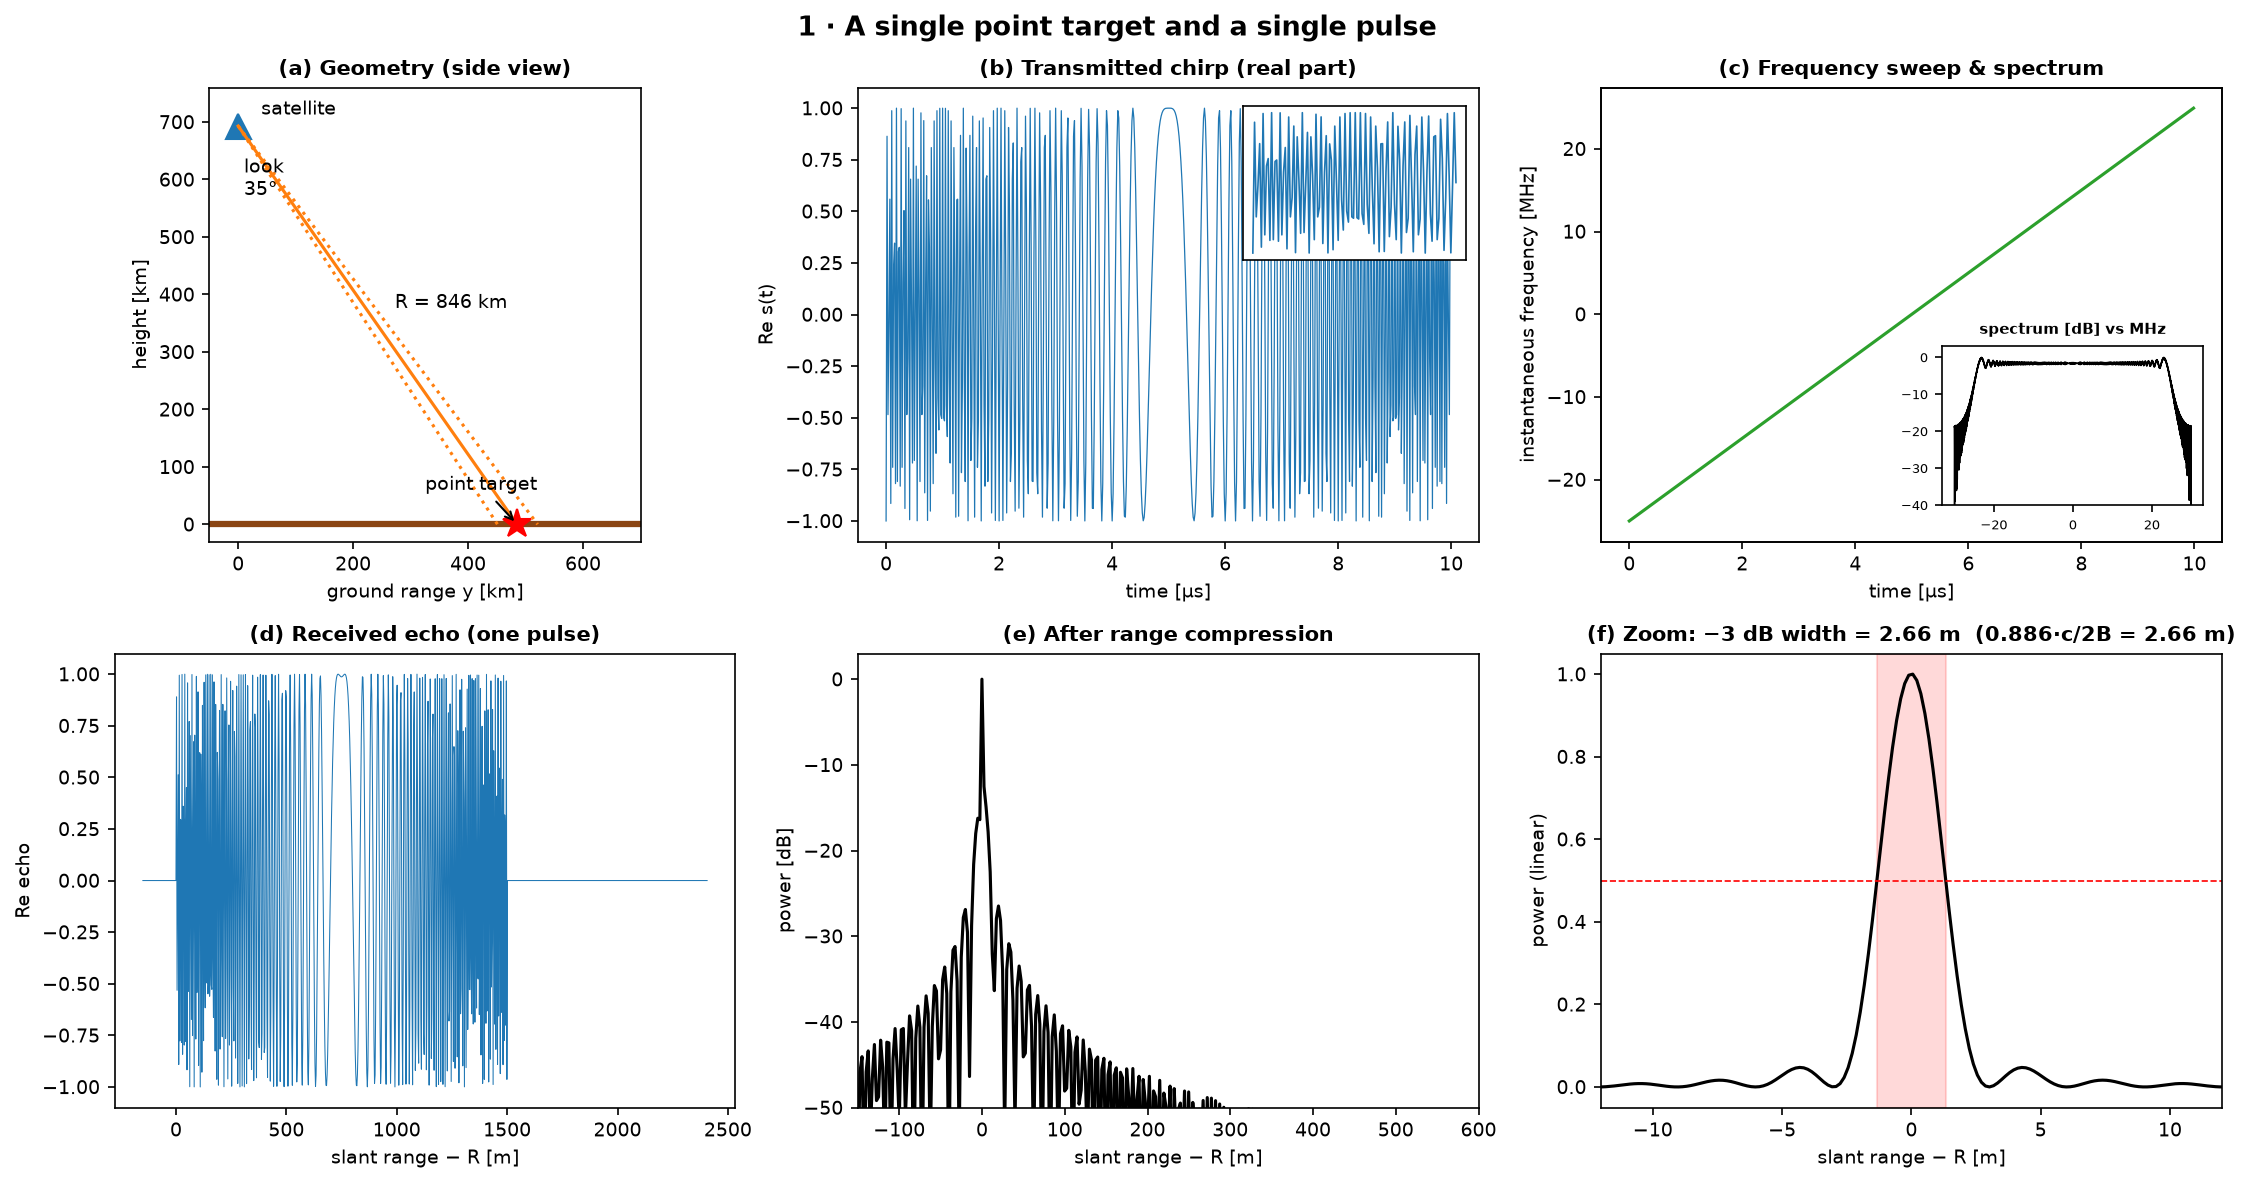
\includegraphics[width=\textwidth]{01_point_single_pulse.png}
\caption[A single point target illuminated by one pulse]{A single point target illuminated by one pulse: (\textbf{a}) geometry; (\textbf{b}) transmitted chirp; (\textbf{c}) frequency sweep and spectrum; (\textbf{d}) received echo; (\textbf{e}) range-compressed signal; (\textbf{f}) $-3$\,dB width of the compressed peak.}
\label{fig:point}
\end{figure}
\begin{figure}[htbp]
\centering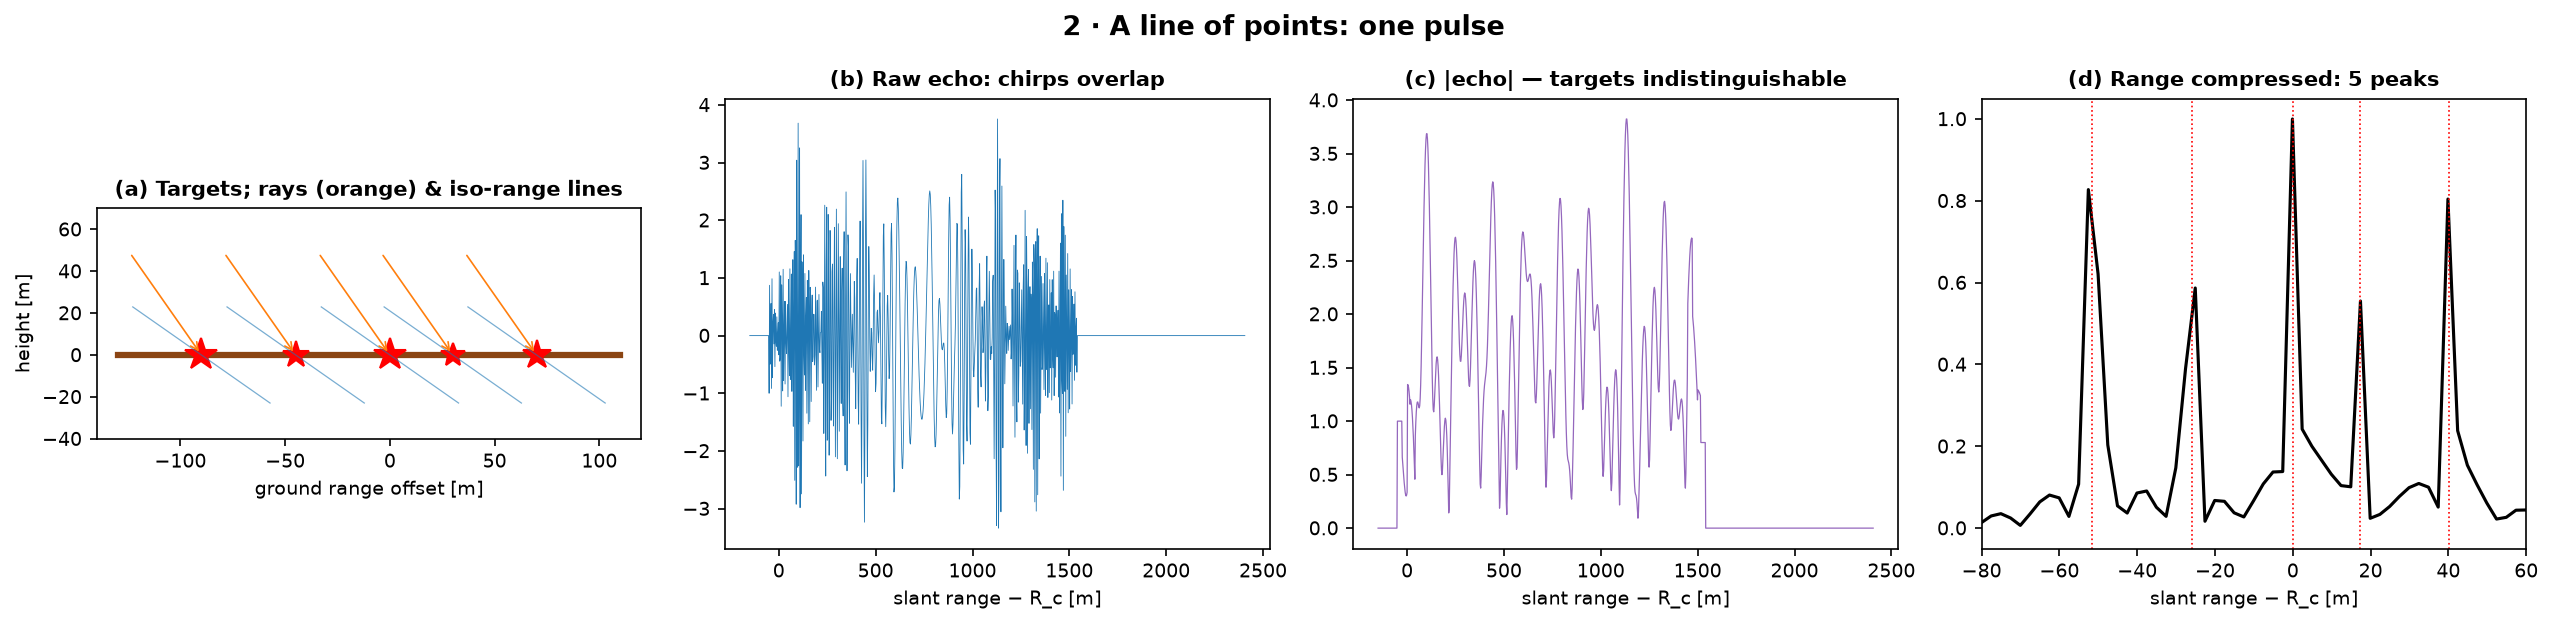
\includegraphics[width=\textwidth]{02_line_of_points.png}\\[2pt]
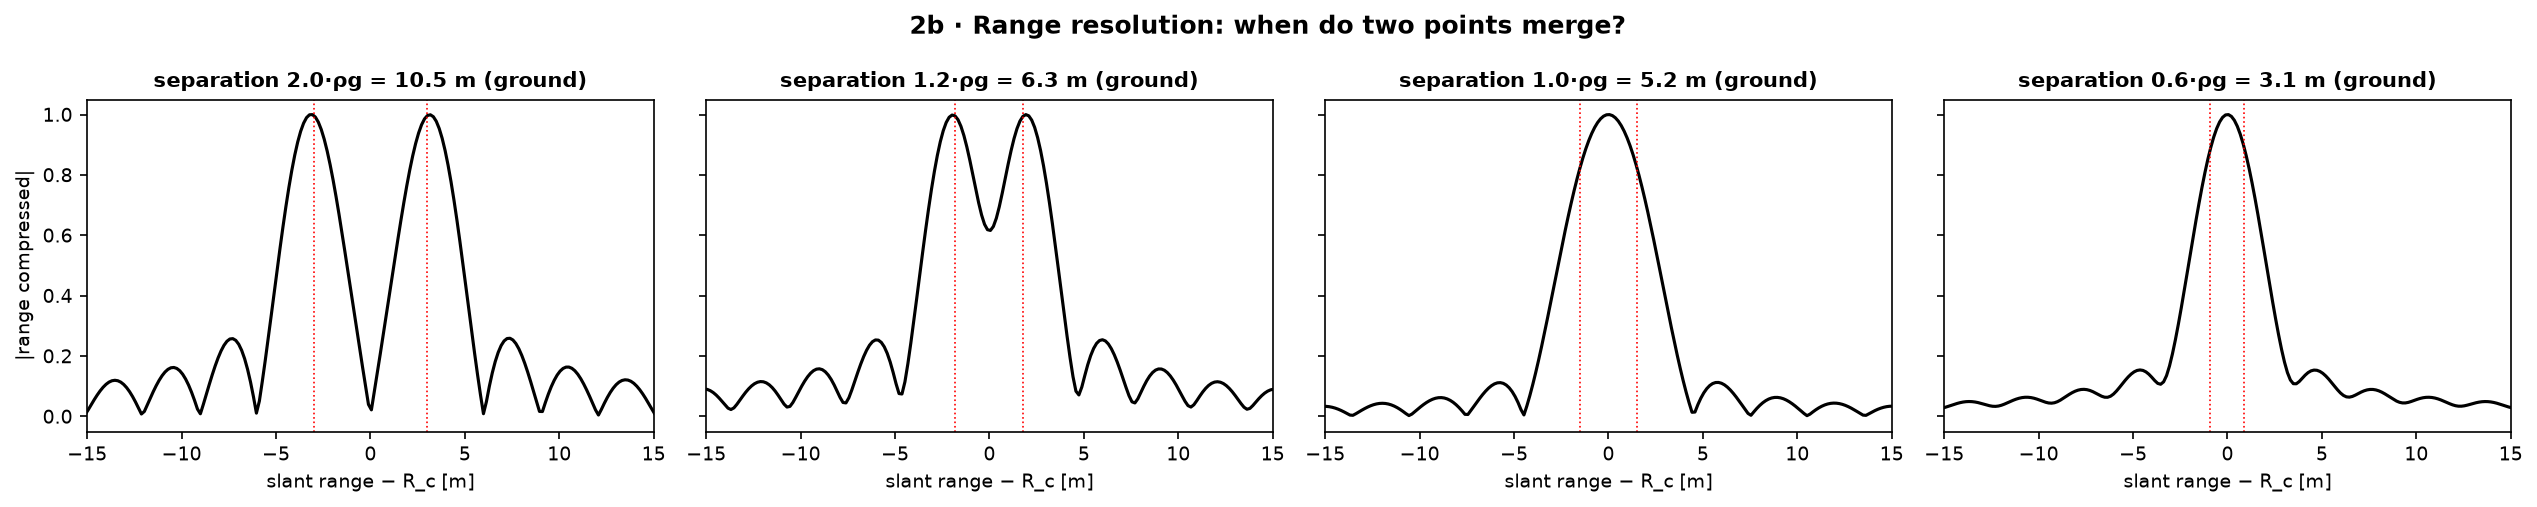
\includegraphics[width=\textwidth]{02b_range_resolution.png}
\caption[A line of point targets and the range resolution]{A line of point targets and the range resolution. Top: five targets on a line, their overlapping echoes and the compressed range profile. Bottom: two equal targets at decreasing separation, expressed in multiples of the ground-range resolution $\rho_g$.}
\label{fig:line}
\end{figure}

Along the synthetic aperture, each target follows a hyperbolic range history and a linear Doppler history (Fig.~\ref{fig:moving}). For the spaceborne geometry the range migration over the processed aperture of 4.6\,km is only 3.2\,m, about one range resolution cell, so that the range-compressed azimuth chirps are nearly straight. Back-projection focuses the three targets at their true positions with measured resolutions of 5.45\,m in azimuth and 4.65\,m in ground range and peak side-lobe ratios of $-23.6$\,dB and $-13.3$\,dB, respectively (Fig.~\ref{fig:irf}); the theoretical values are $L/2=6.15$\,m and $0.886\,\rho_r/\sin\theta=4.63$\,m. The lower azimuth side-lobes result from the antenna pattern, which acts as a taper.

\begin{figure}[htbp]
\centering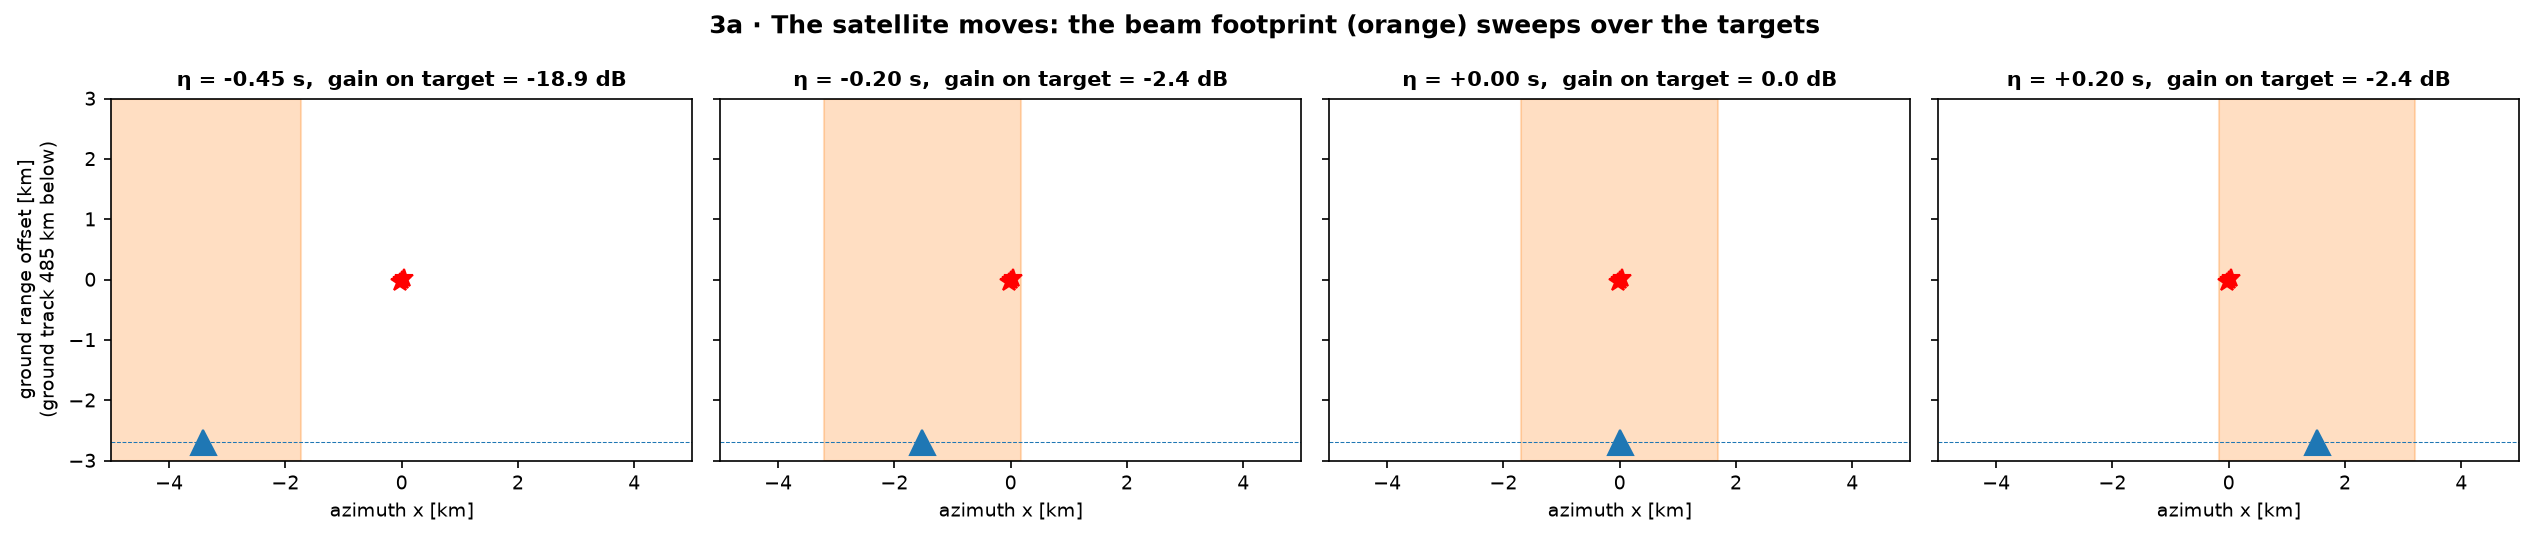
\includegraphics[width=\textwidth]{03a_moving_satellite_snapshots.png}\\[2pt]
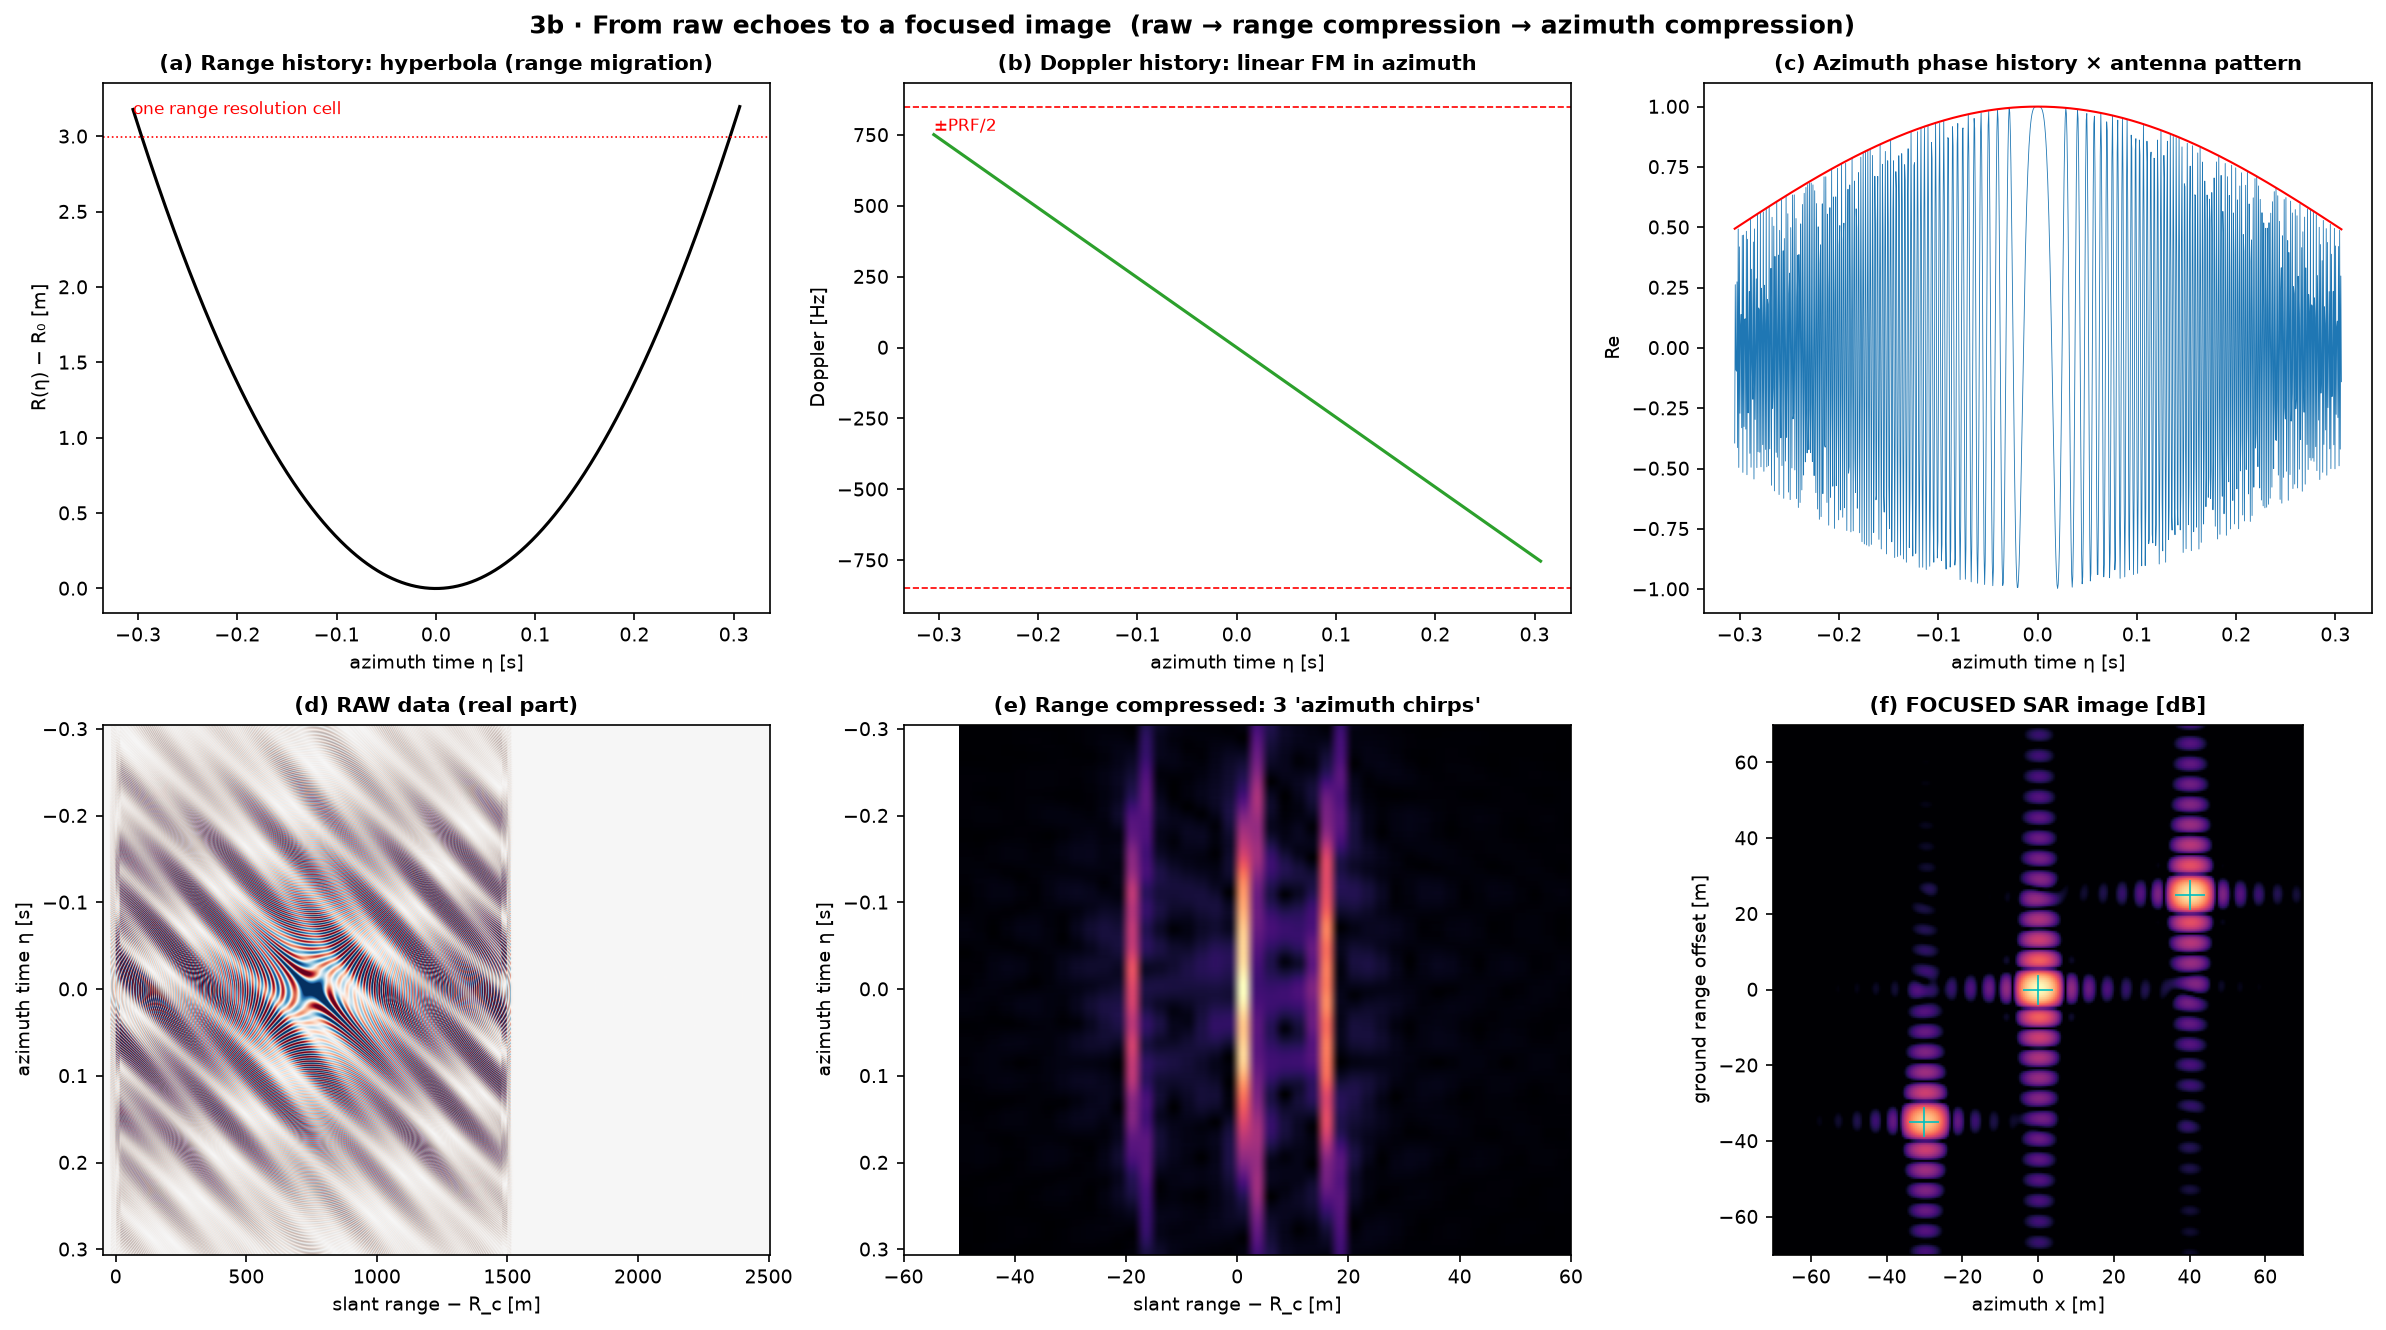
\includegraphics[width=\textwidth]{03b_signal_chain.png}
\caption[Formation of the synthetic aperture]{Formation of the synthetic aperture. Top: the beam footprint passing over three targets. Bottom: (\textbf{a}) range history; (\textbf{b}) Doppler history; (\textbf{c}) azimuth phase history weighted by the antenna pattern; (\textbf{d}) raw data; (\textbf{e}) range-compressed data; (\textbf{f}) focused image.}
\label{fig:moving}
\end{figure}
\begin{figure}[htbp]
\centering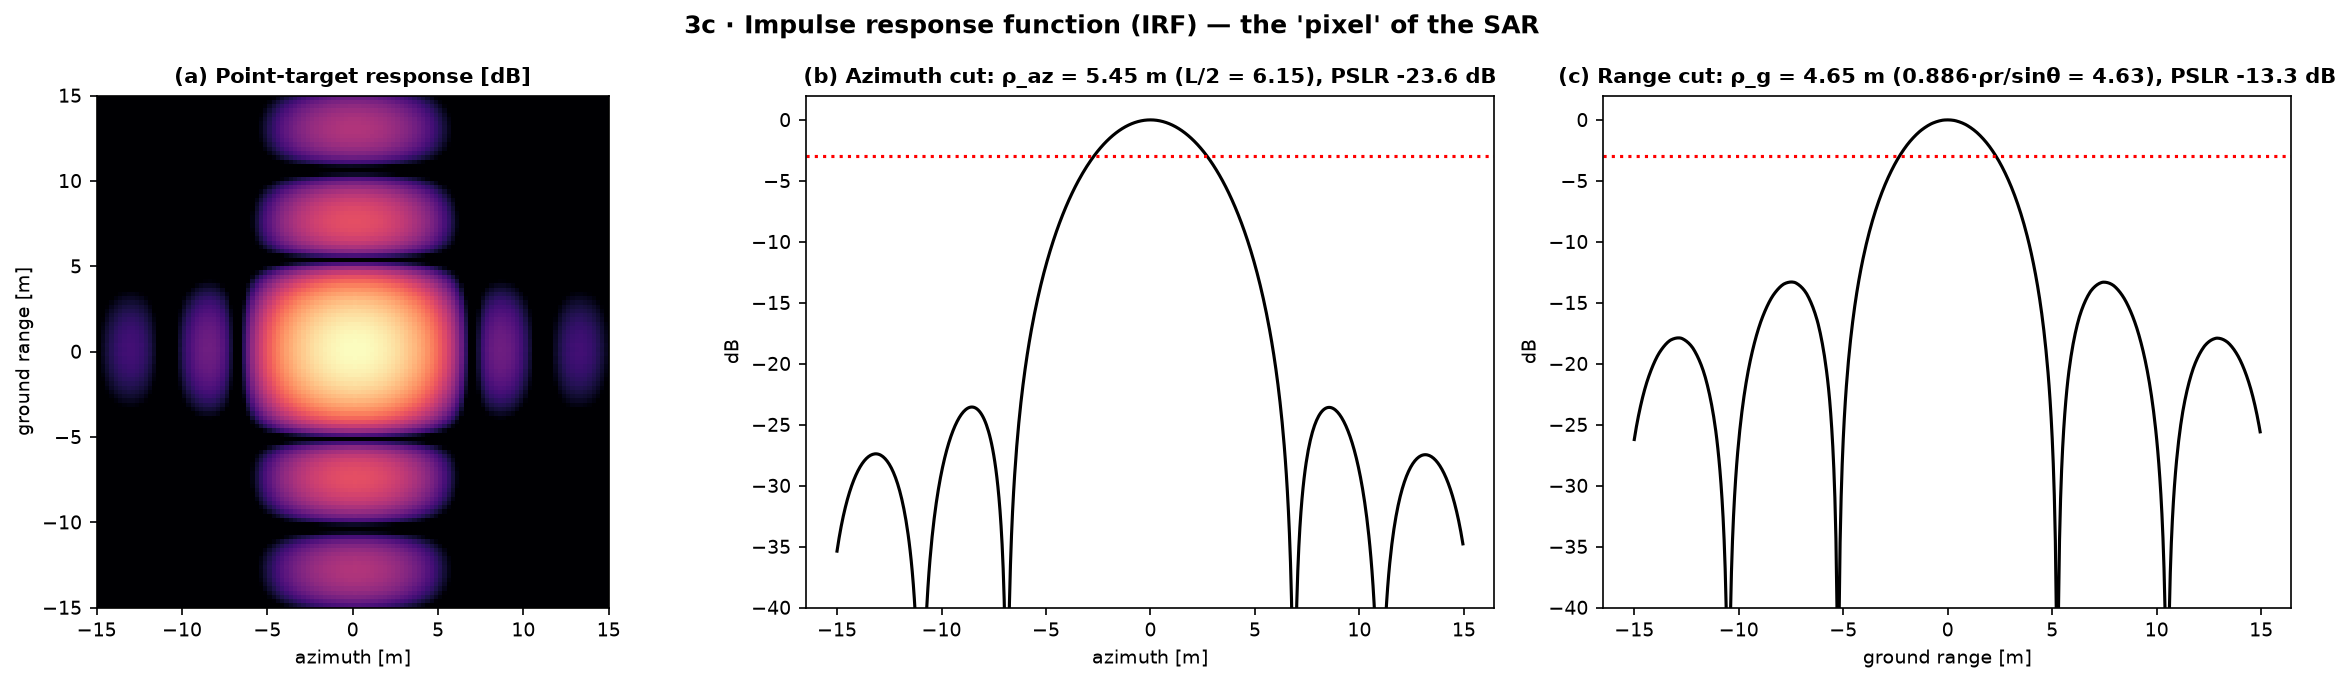
\includegraphics[width=\textwidth]{03c_impulse_response.png}
\caption[Impulse response function of the simulated SAR and its cuts in azimuth and ground range]{Impulse response function of the simulated SAR (\textbf{a}) and its cuts in azimuth (\textbf{b}) and ground range (\textbf{c}).}
\label{fig:irf}
\end{figure}

A field of 4941 scatterers with circular Gaussian amplitudes produces raw data without visible structure and a focused image that consists of fully developed speckle (Fig.~\ref{fig:flat}). The single-look intensity follows the exponential distribution, and multilooking produces a Gamma distribution whose equivalent number of looks agrees with the number of independent resolution cells averaged~\cite{goodman1976,oliver1998}. For a sinusoidal surface with uniform reflectivity per unit ground area (amplitude 12\,m, period 150\,m), the focused image still shows bright bands on the slopes facing the radar (Fig.~\ref{fig:sine}); the azimuth-averaged profile of the raw-signal simulation is reproduced by the image-domain simulation with $r=0.90$, the residual being speckle. On the $480\times480$\,m DEM patch (relief of about 550\,m; about 15{,}000 scatterers and 1100 pulses), the raw-signal simulation and focusing take about 100\,s and the image-domain simulation about 30\,ms; after $9\times9$ multilooking both agree with $r=0.97$ (Fig.~\ref{fig:dempatch}). The image-domain simulator was therefore adopted for scene-scale simulations (Fig.~\ref{fig:design}, iteration 4).

\begin{figure}[htbp]
\centering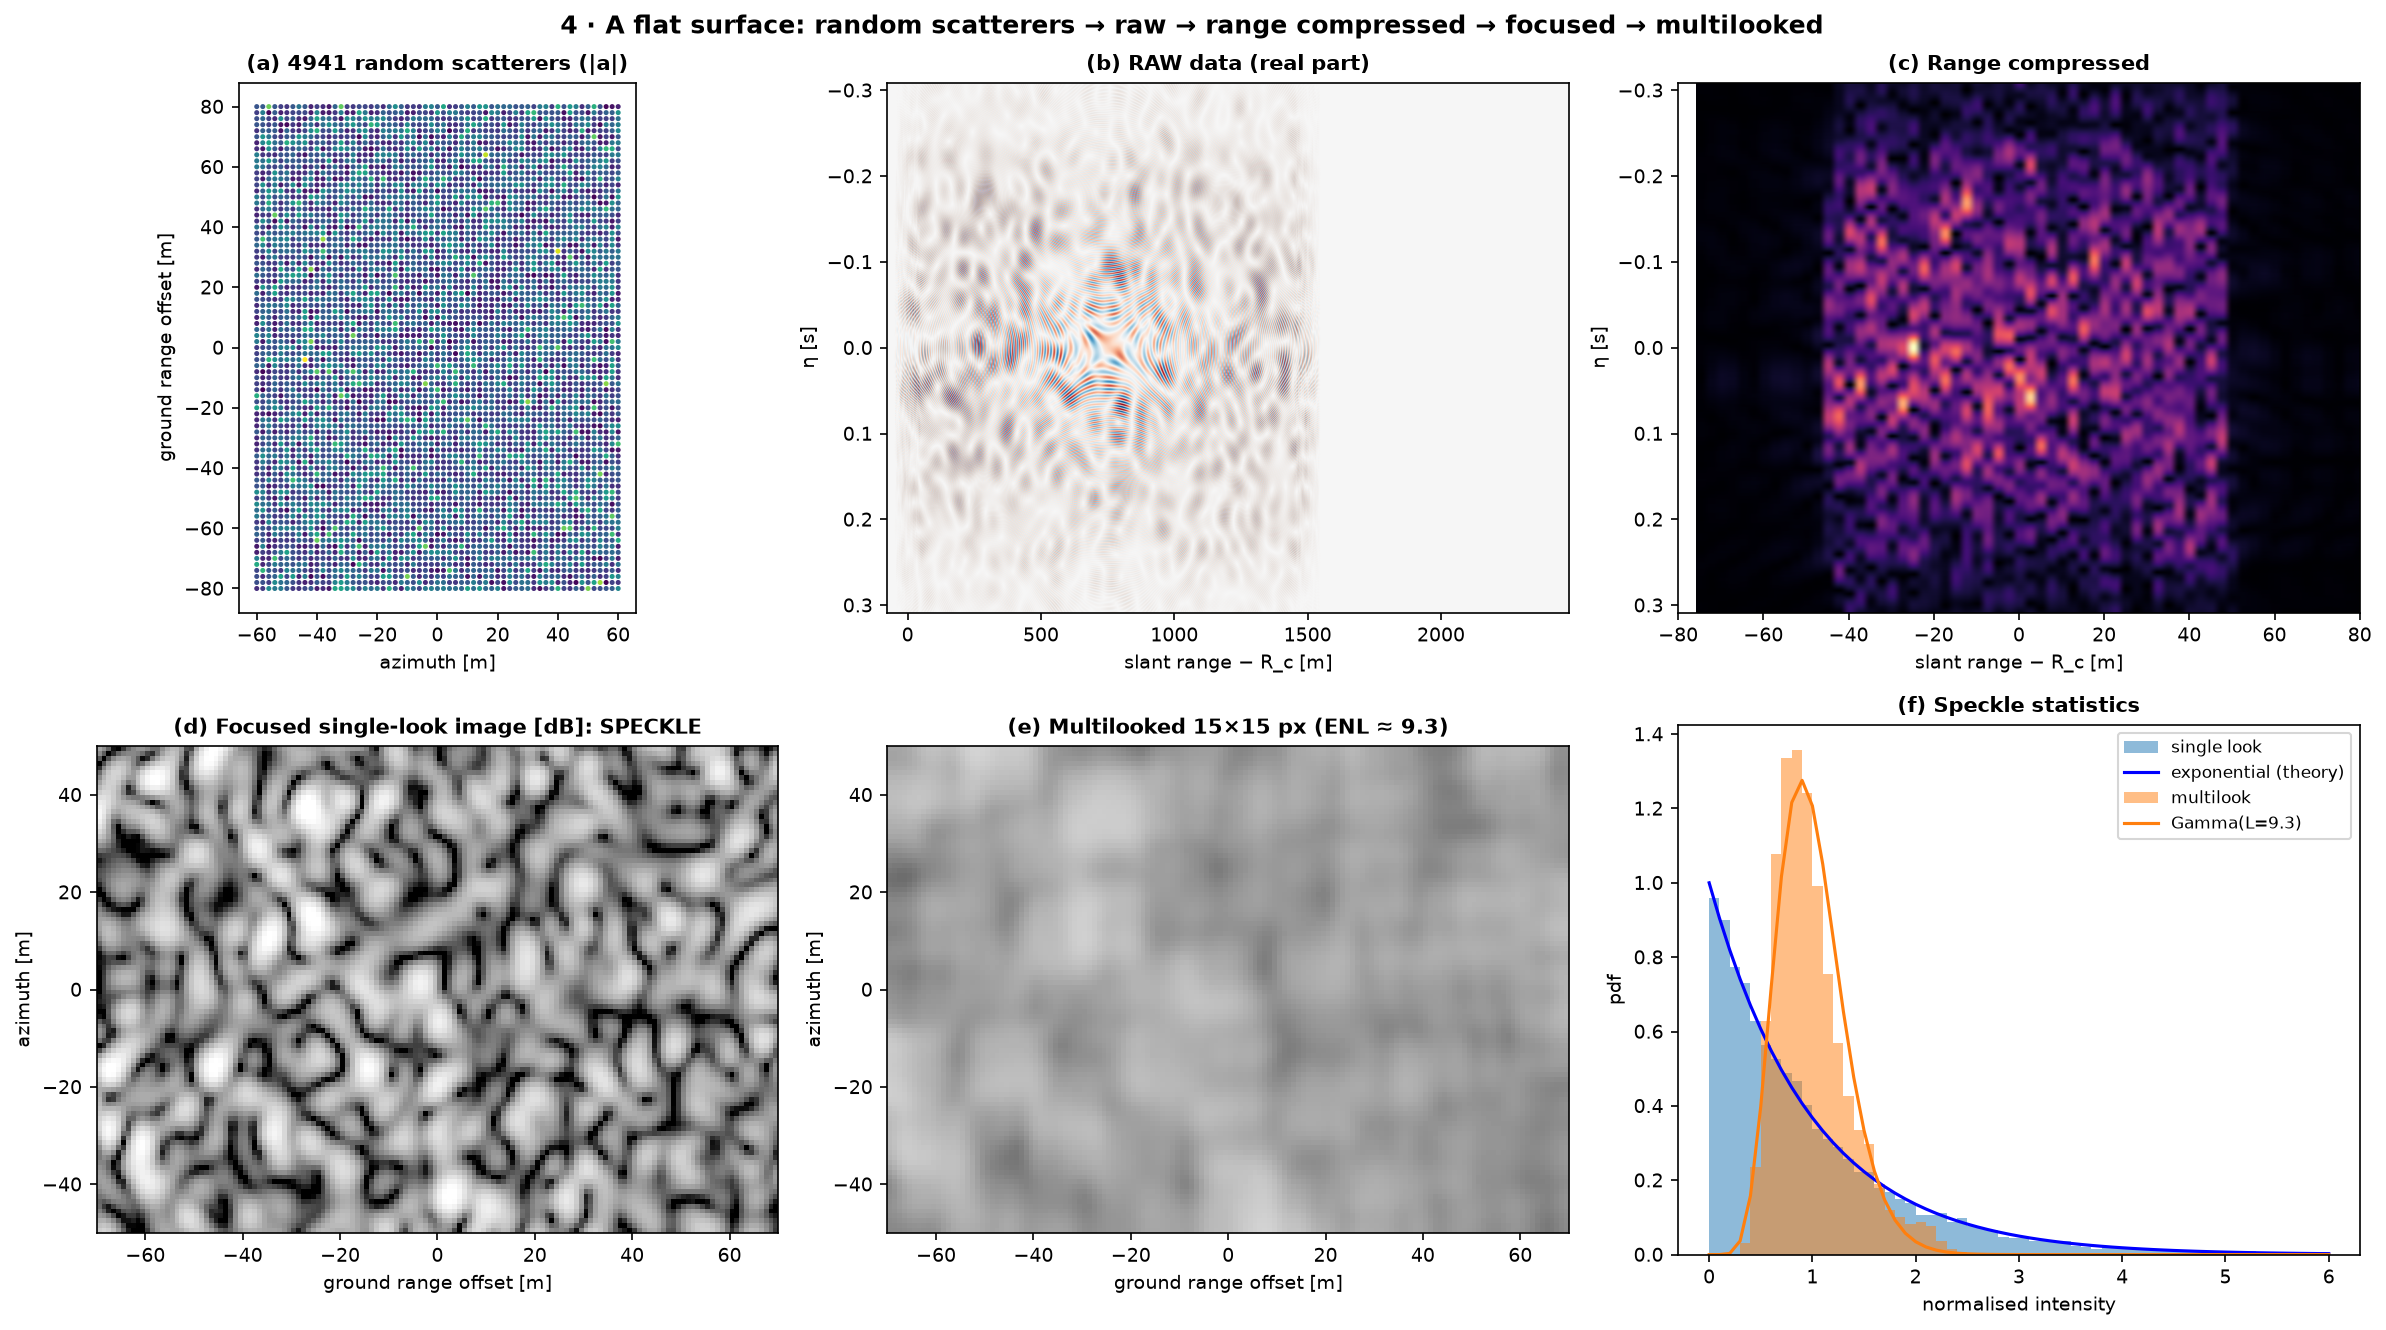
\includegraphics[width=\textwidth]{04_flat_surface_speckle.png}
\caption[Distributed scatterers]{Distributed scatterers: (\textbf{a}) random scatterer field; (\textbf{b}) raw data; (\textbf{c}) range-compressed data; (\textbf{d}) focused single-look image; (\textbf{e}) multilooked image; (\textbf{f}) intensity statistics compared with the exponential and Gamma distributions.}
\label{fig:flat}
\end{figure}
\begin{figure}[htbp]
\centering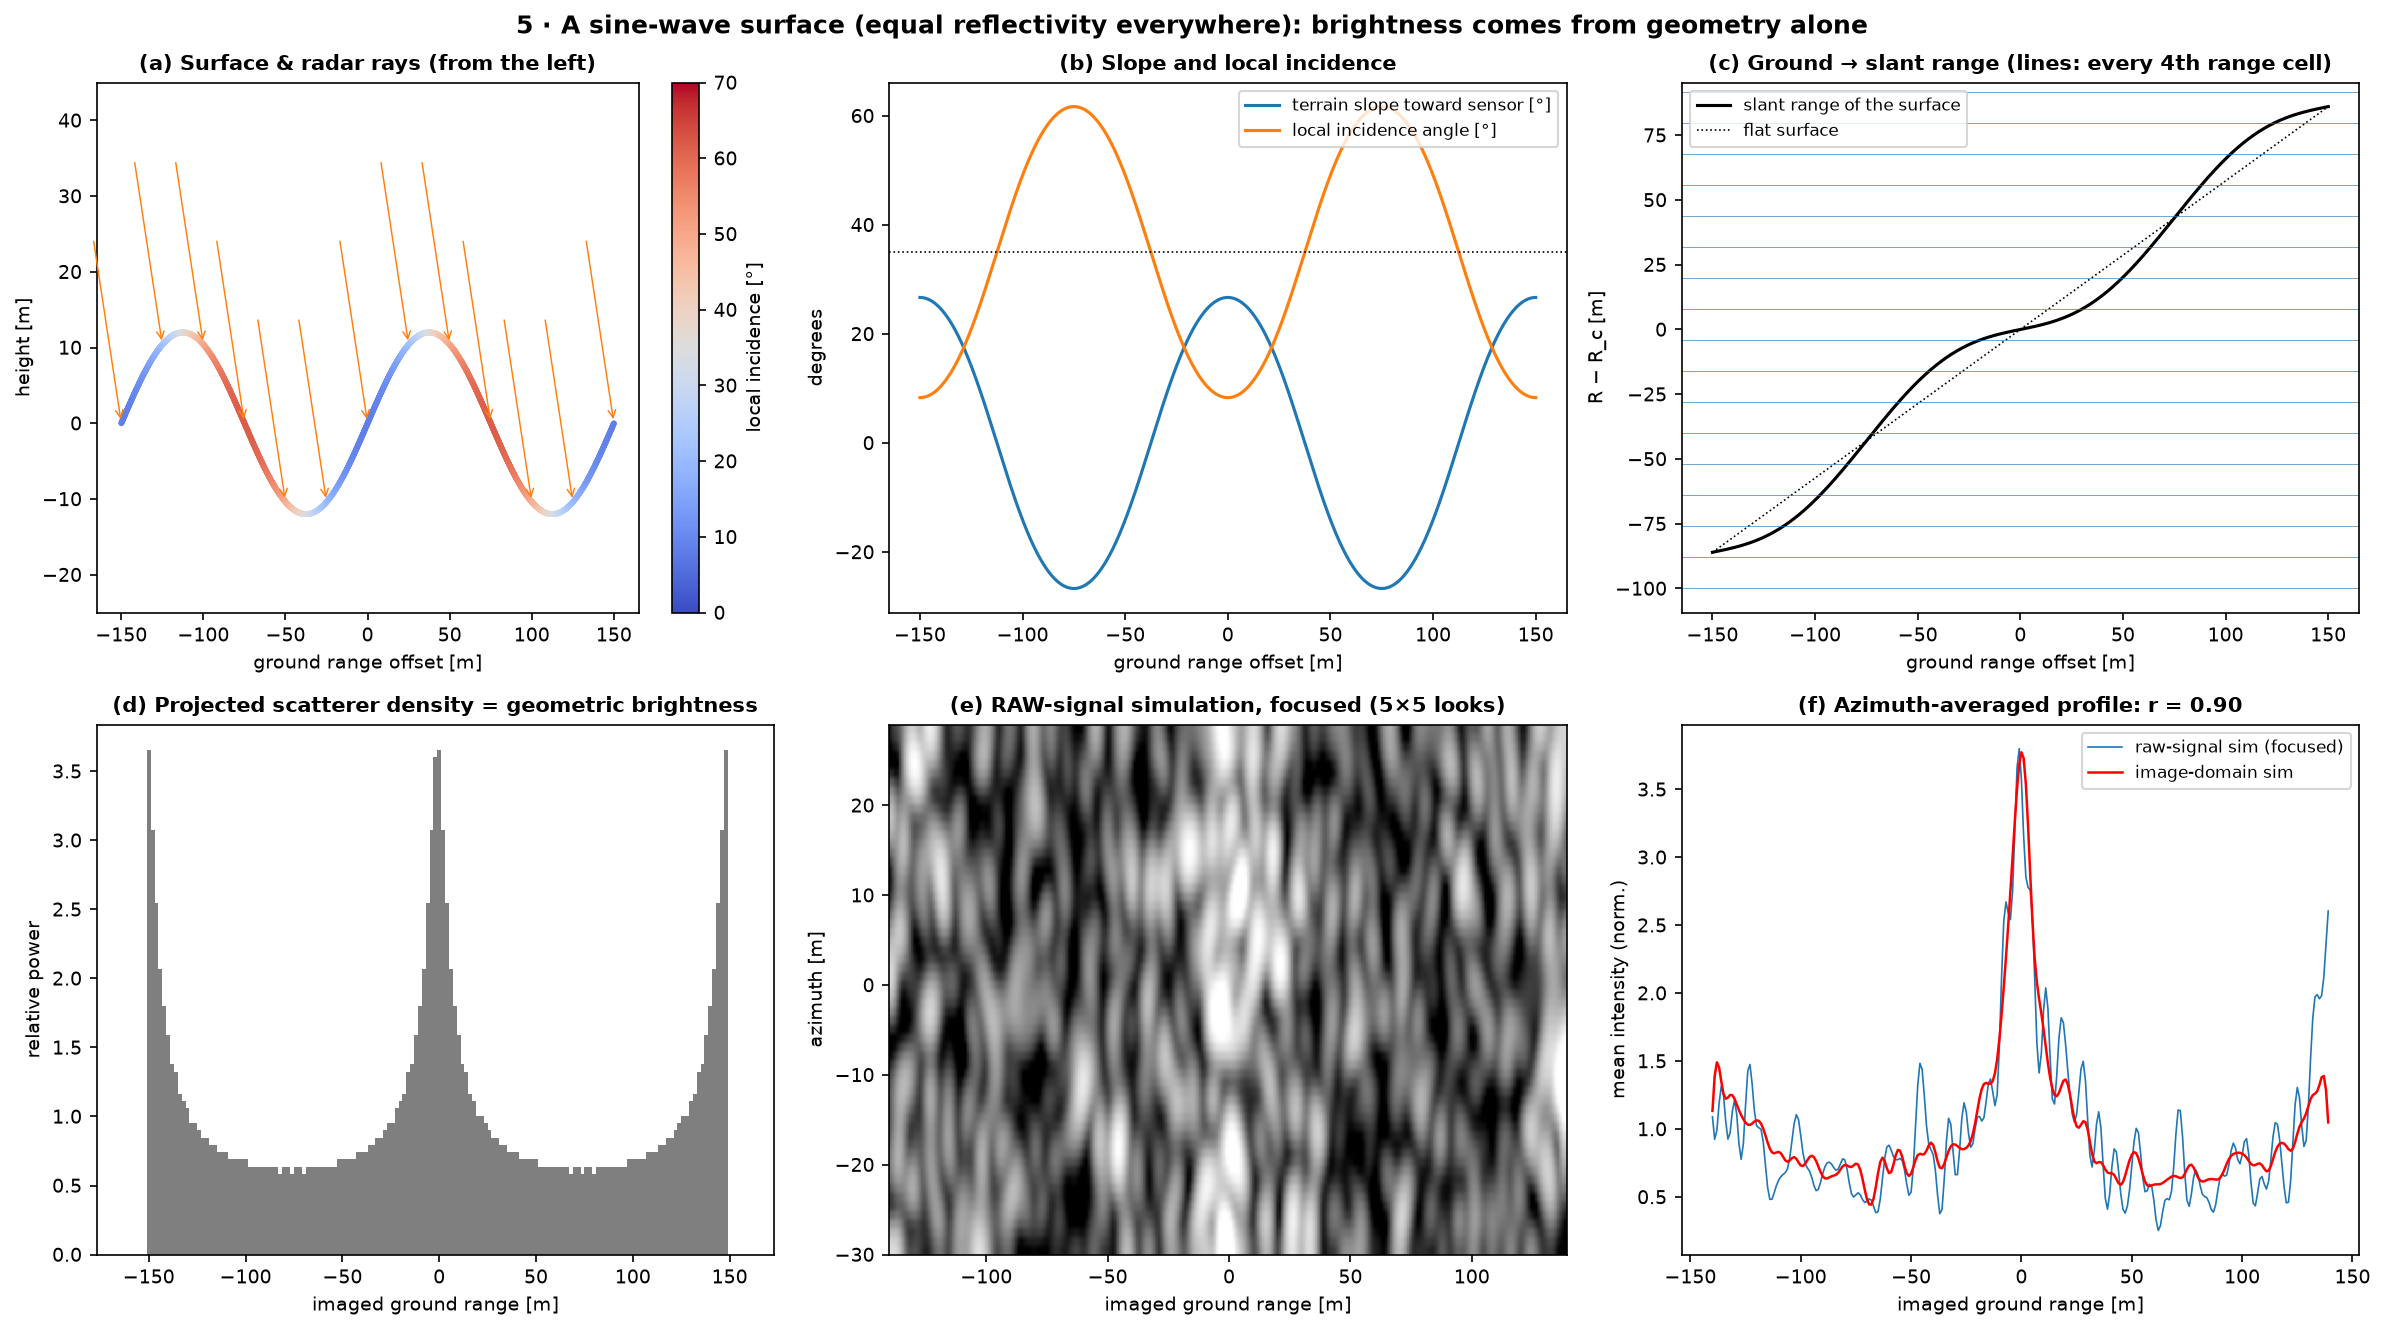
\includegraphics[width=\textwidth]{05_sine_surface.png}
\caption[Sinusoidal surface with uniform reflectivity]{Sinusoidal surface with uniform reflectivity: (\textbf{a}) profile and radar rays; (\textbf{b}) slope and local incidence angle; (\textbf{c}) ground-to-slant-range mapping; (\textbf{d}) projected scatterer density; (\textbf{e}) focused raw-signal simulation; (\textbf{f}) azimuth-averaged profiles of the raw-signal and image-domain simulations.}
\label{fig:sine}
\end{figure}
\begin{figure}[htbp]
\centering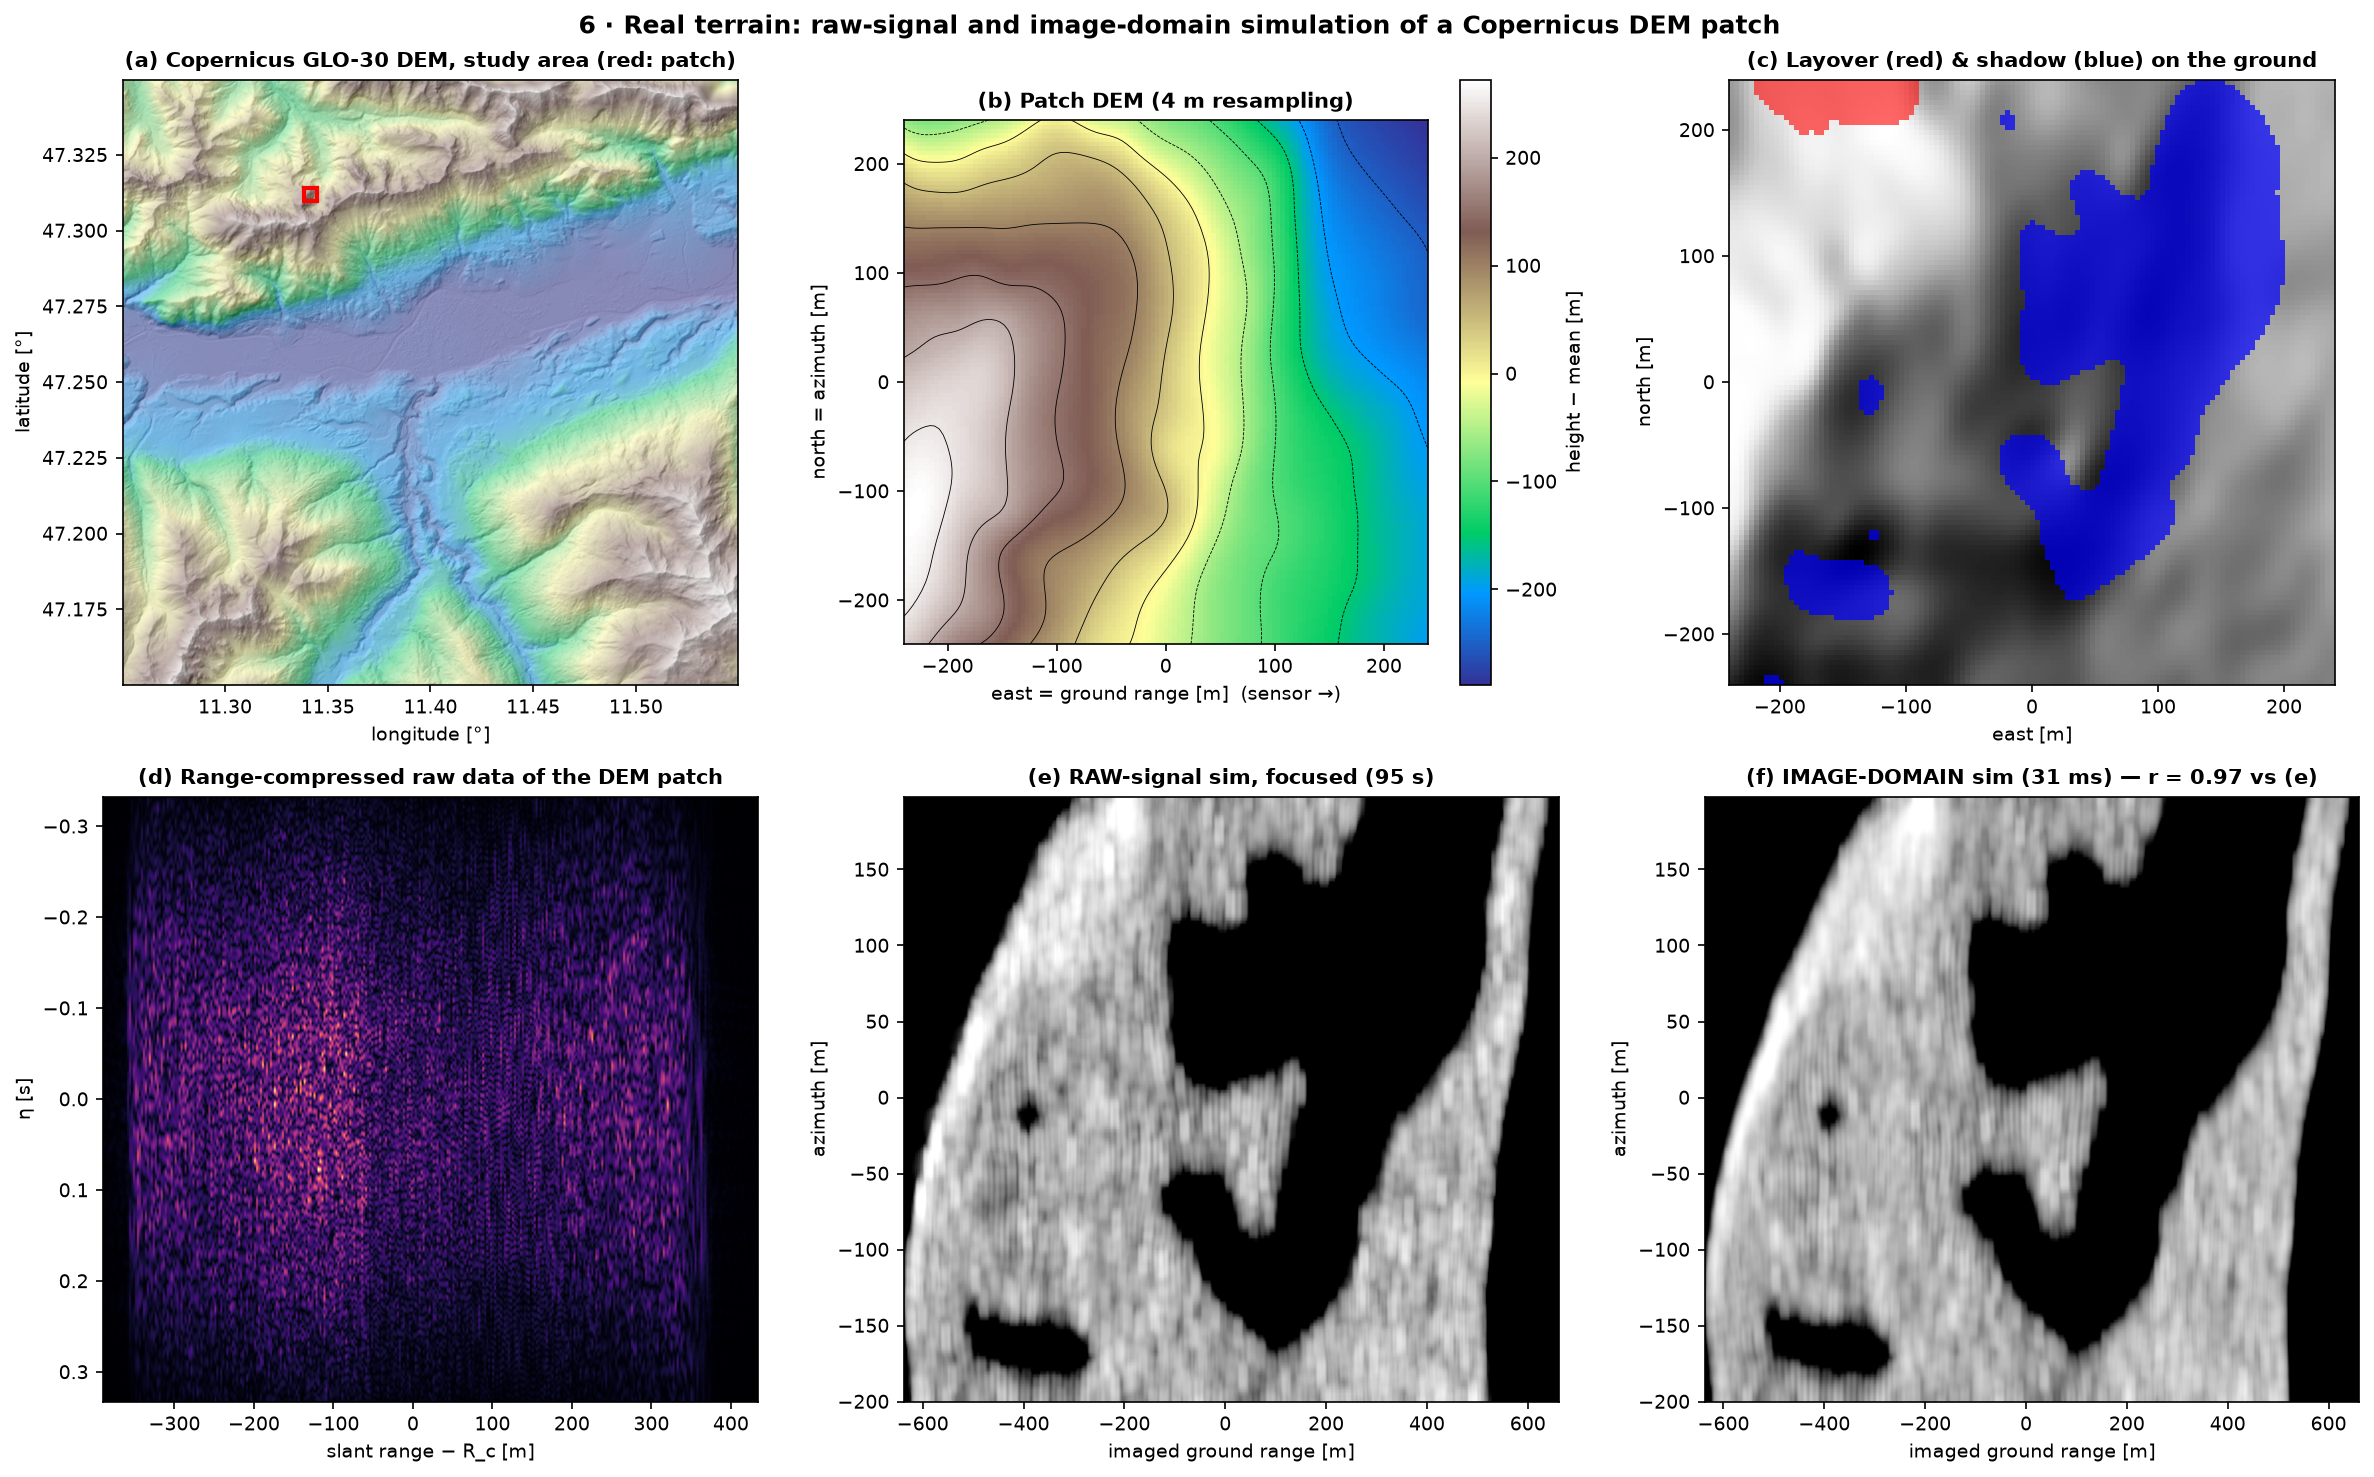
\includegraphics[width=\textwidth]{06_dem_patch_raw_vs_image_domain.png}
\caption[Copernicus DEM patch]{Copernicus DEM patch: (\textbf{a}) location; (\textbf{b}) patch DEM; (\textbf{c}) layover and shadow on the ground; (\textbf{d}) range-compressed raw data; (\textbf{e}) focused raw-signal simulation; (\textbf{f}) image-domain simulation.}
\label{fig:dempatch}
\end{figure}

\section{Geometric Distortions over the Study Site}
On a synthetic profile with a 55$^\circ$ fore-slope and a 65$^\circ$ back-slope observed at a 35$^\circ$ look angle, the shadow and layover criteria classify the fore-slope as active layover, the valley floor in front of it as passive layover, the back-slope and the plain behind it as shadow, and a gentle hill with a maximum slope of about 20$^\circ$ as foreshortened only (Fig.~\ref{fig:geomprofile}). On a $9\times9$\,km subset of the study site, layover affects 18\,\% of the area at a look angle of 20$^\circ$ and decreases to about 1\,\% at 50$^\circ$, while shadow increases from 0 to 3.4\,\% (Fig.~\ref{fig:geomdem}), which illustrates the classical trade-off in the choice of incidence angle over mountains~\cite{kropatsch1990,gelautz1998}. Fig.~\ref{fig:radio} builds the simulated image in the order of the physics: local incidence angle, $\sigz(\theta_{loc})$, illuminated area, their product, speckle and multilooking. The geometric term alone, i.e., the illuminated area per pixel, already reproduces most of the image structure.

\begin{figure}[htbp]
\centering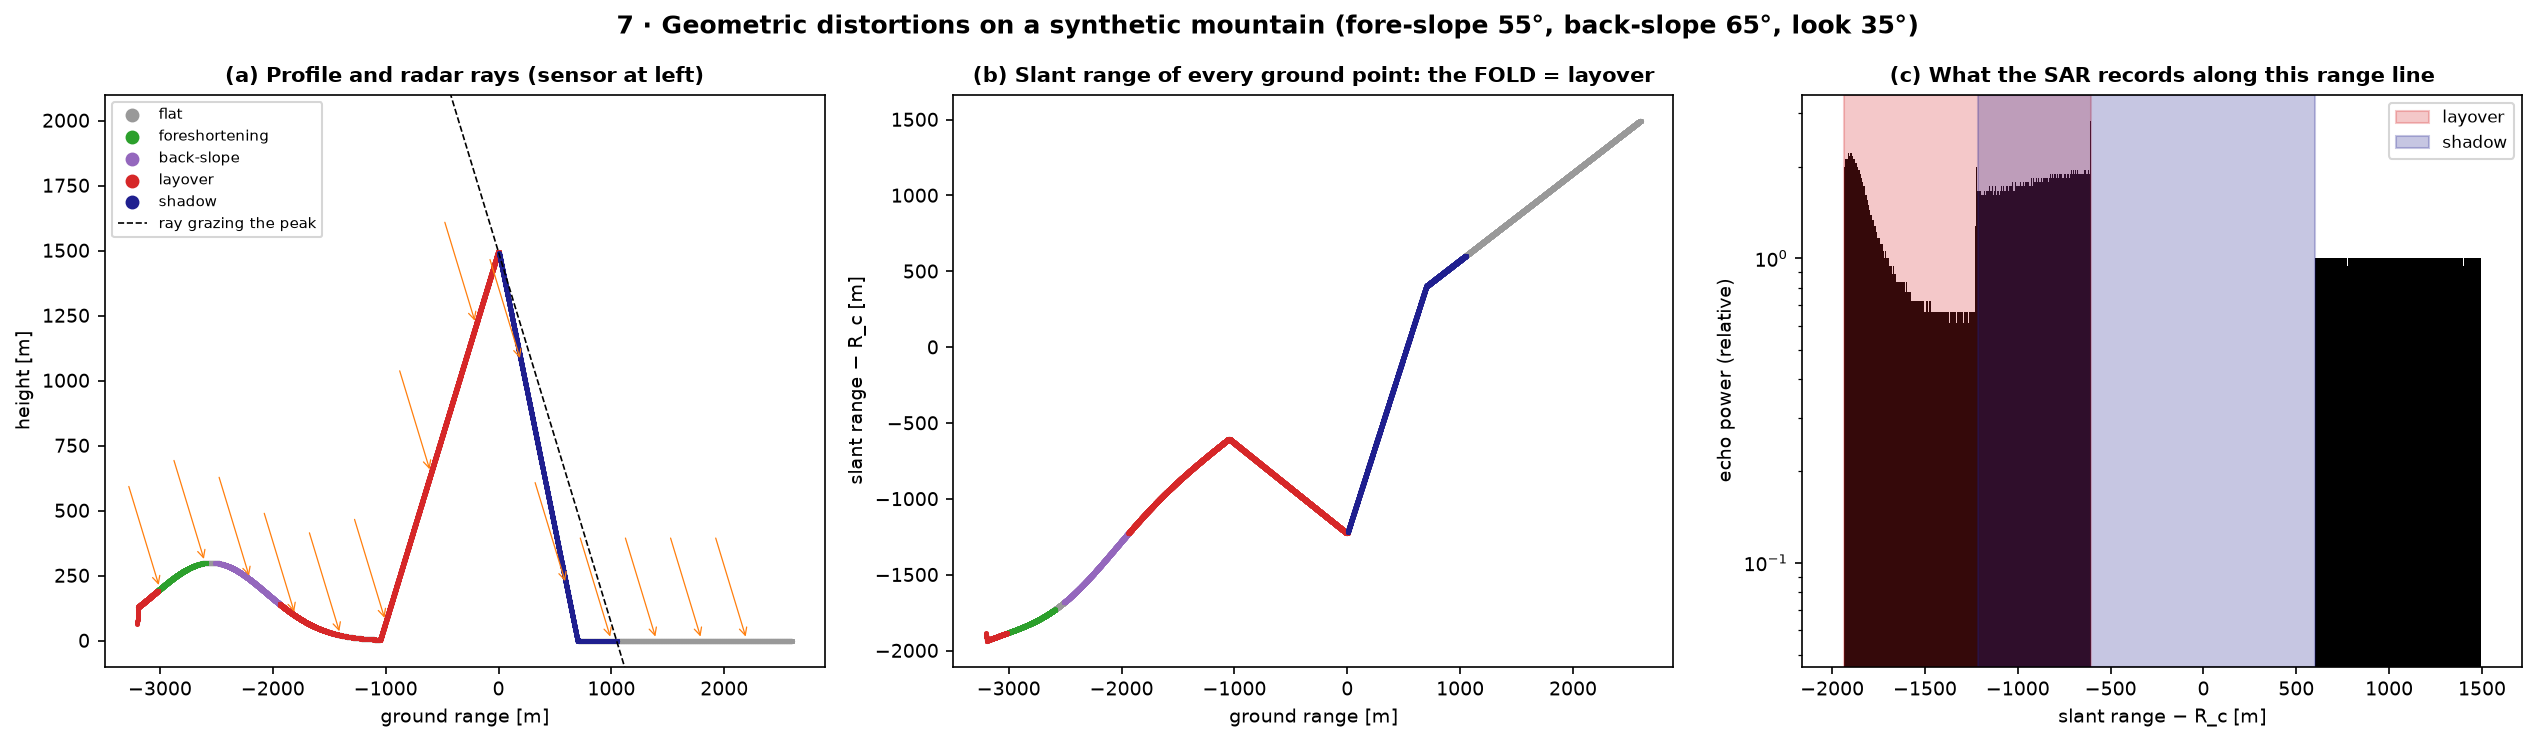
\includegraphics[width=\textwidth]{07_geometric_distortions_profile.png}
\caption[Geometric distortions along a synthetic profile]{Geometric distortions along a synthetic profile: (\textbf{a}) classification and radar rays; (\textbf{b}) slant range of every ground point, where the fold indicates layover; (\textbf{c}) echo power recorded along the range line.}
\label{fig:geomprofile}
\end{figure}
\begin{figure}[htbp]
\centering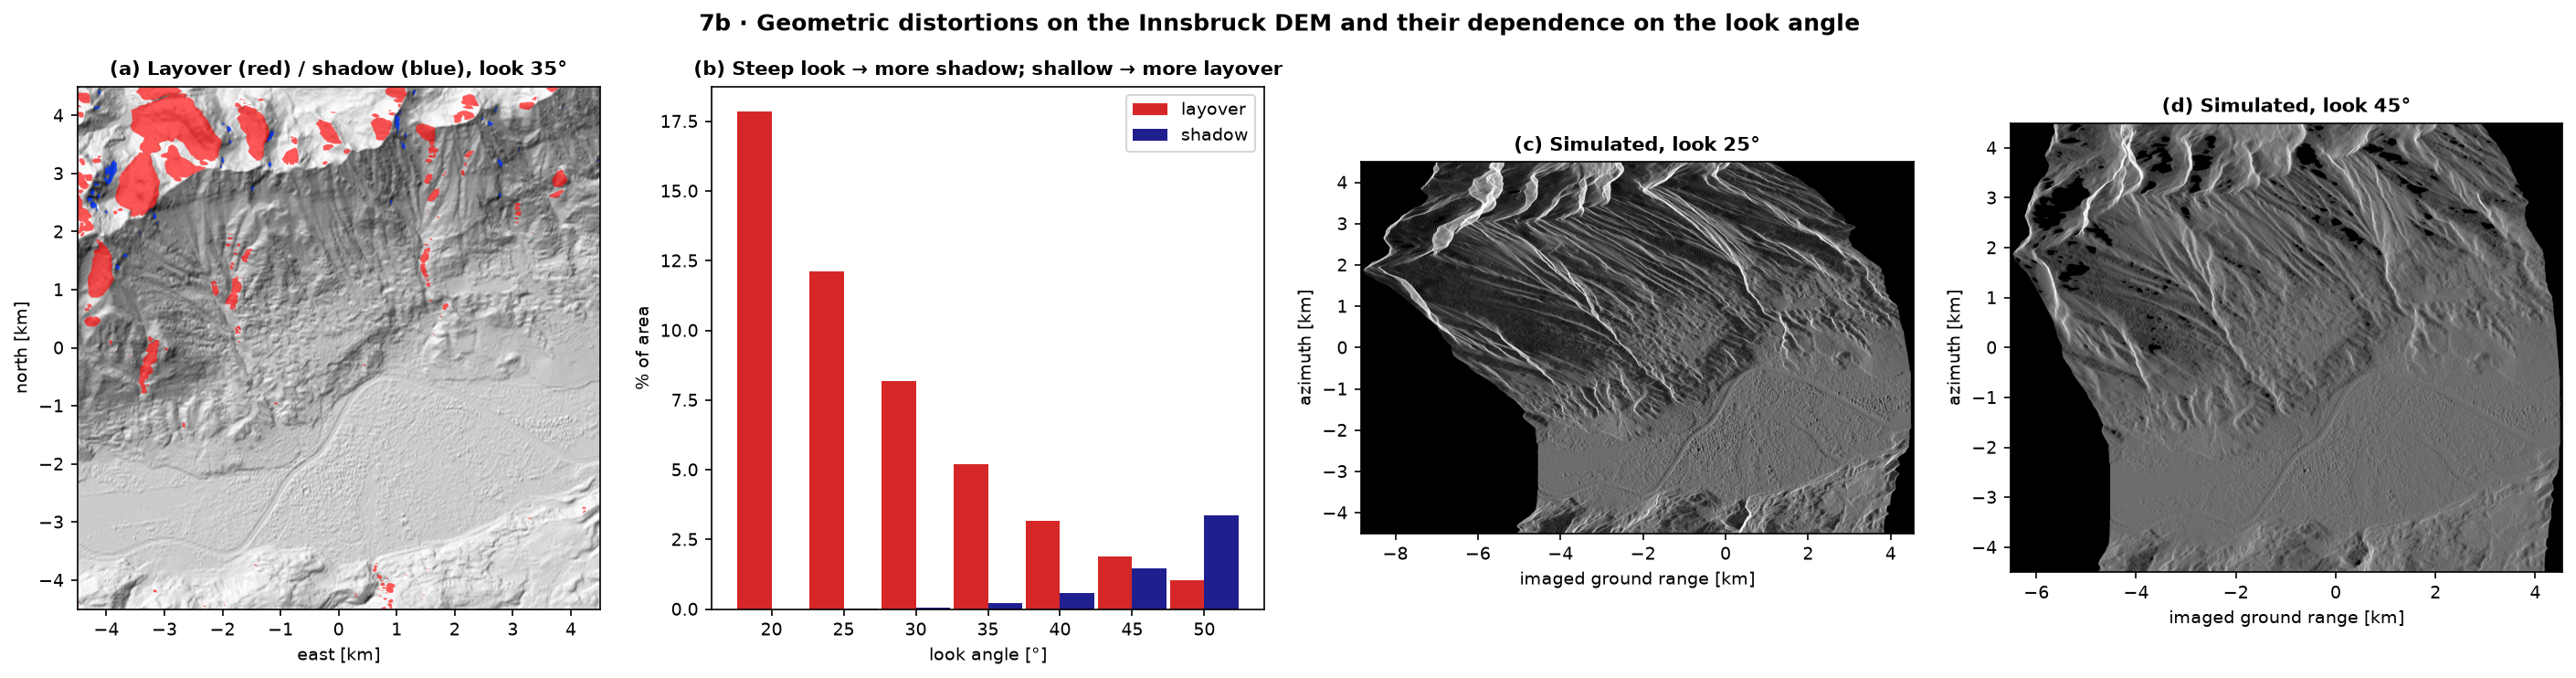
\includegraphics[width=\textwidth]{07b_geometric_distortions_dem.png}
\caption[Layover and shadow over a $9\times9$\,km subset of the study site, their fraction as a function of the look angle, and simulated images at look angles of 25$^\circ$ and 45$^\circ$]{Layover and shadow over a $9\times9$\,km subset of the study site (\textbf{a}), their fraction as a function of the look angle (\textbf{b}), and simulated images at look angles of 25$^\circ$ (\textbf{c}) and 45$^\circ$ (\textbf{d}).}
\label{fig:geomdem}
\end{figure}
\begin{figure}[htbp]
\centering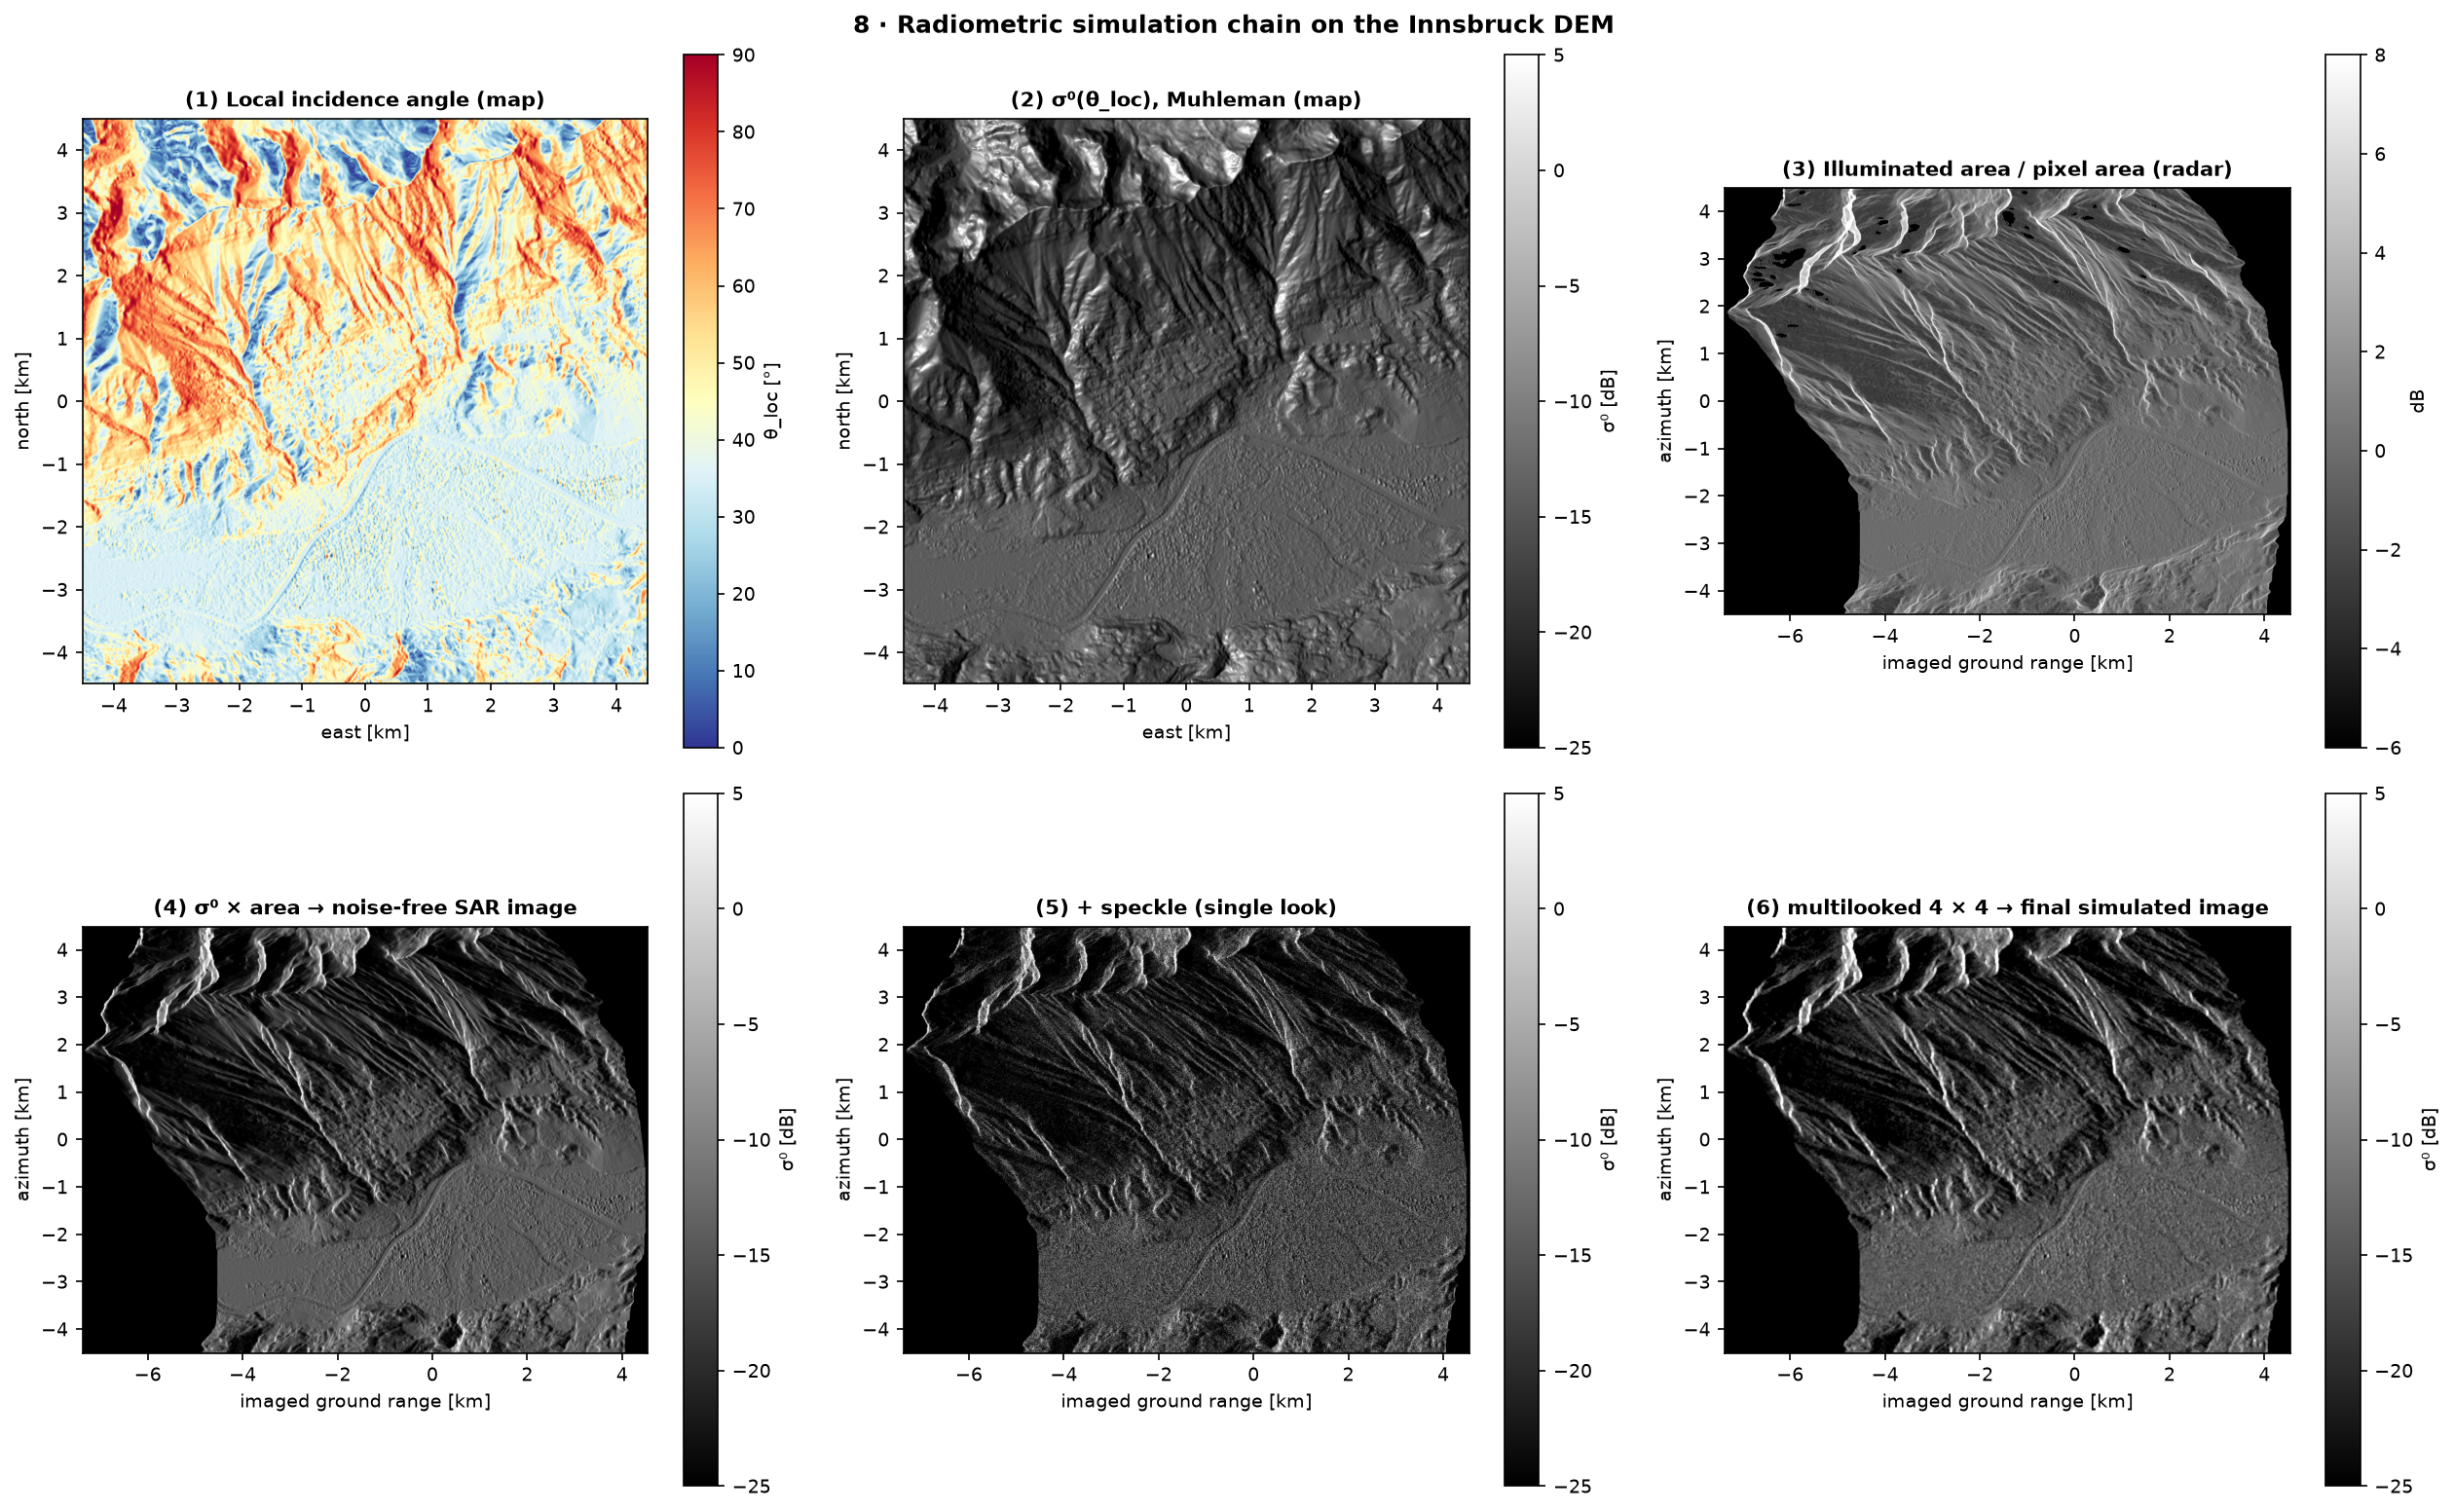
\includegraphics[width=\textwidth]{08b_radiometric_chain.png}
\caption[Radiometric simulation chain]{Radiometric simulation chain: (\textbf{1}) local incidence angle; (\textbf{2}) $\sigz$ from Muhleman's law in map geometry; (\textbf{3}) illuminated area per pixel in radar geometry; (\textbf{4}) noise-free simulated image; (\textbf{5}) single-look speckle; (\textbf{6}) multilooked image.}
\label{fig:radio}
\end{figure}

\section{Geocoding Accuracy}
\label{sec:res-geo}
With the valid-from rule for the SRGR polynomials, the range-Doppler geocoding reproduces the geolocation grid of both products to \geoDpixMax{} pixels in range, \geoDtMax{} ms in zero-Doppler time (\geoDlineMax{} lines) and \geoDRmax{} mm in slant range over all \nGrid{} tie points of each scene (Fig.~\ref{fig:geomval}a). Linear interpolation between the polynomial sets increased the maximum range error to 3.3 pixels (Fig.~\ref{fig:design}, iteration 5). The line numbers tabulated in the geolocation grid are nominal and deviate by up to 0.2 lines from the zero-Doppler times listed for the same points; the latter must be used for validation.

\section{Comparison with Sentinel-1 and the Backscatter Law}
Fig.~\ref{fig:realsim} compares the real ascending image with the simulation. Ridges, valleys, bright fore-slopes, layover bands and black shadows of the real image are reproduced at the right positions, while the urbanised valley floor appears as a uniform surface in the simulation. Table~\ref{tab:models} and Fig.~\ref{fig:models} summarise the agreement for the five backscatter laws. The constant law, which only contains the illuminated-area term, already reaches $r=0.53$. Laws that decrease with $\theta_{loc}$ improve the agreement substantially, but no single law is best for every metric: Muhleman's law gives the highest correlation ($r=\rMuAsc$), the Lambert and fitted laws the highest SSIM, and the cosine law the lowest RMSE. The fitted law has an exponent $n=\nFit$ and $10\log_{10}k=\kFitDb$\,dB, i.e., the data select Lambert's law (Fig.~\ref{fig:fit}). It describes the median real $\sigz$ well between 10$^\circ$ and 80$^\circ$, whereas at small local incidence angles the real backscatter rises more steeply, which Muhleman's law captures; these few very bright pixels weigh heavily in the Pearson correlation. The interquartile range of the real $\sigz$ at a given $\theta_{loc}$ is about 5\,dB, which indicates that land cover, rather than the angular law, limits the agreement.

\begin{figure}[htbp]
\centering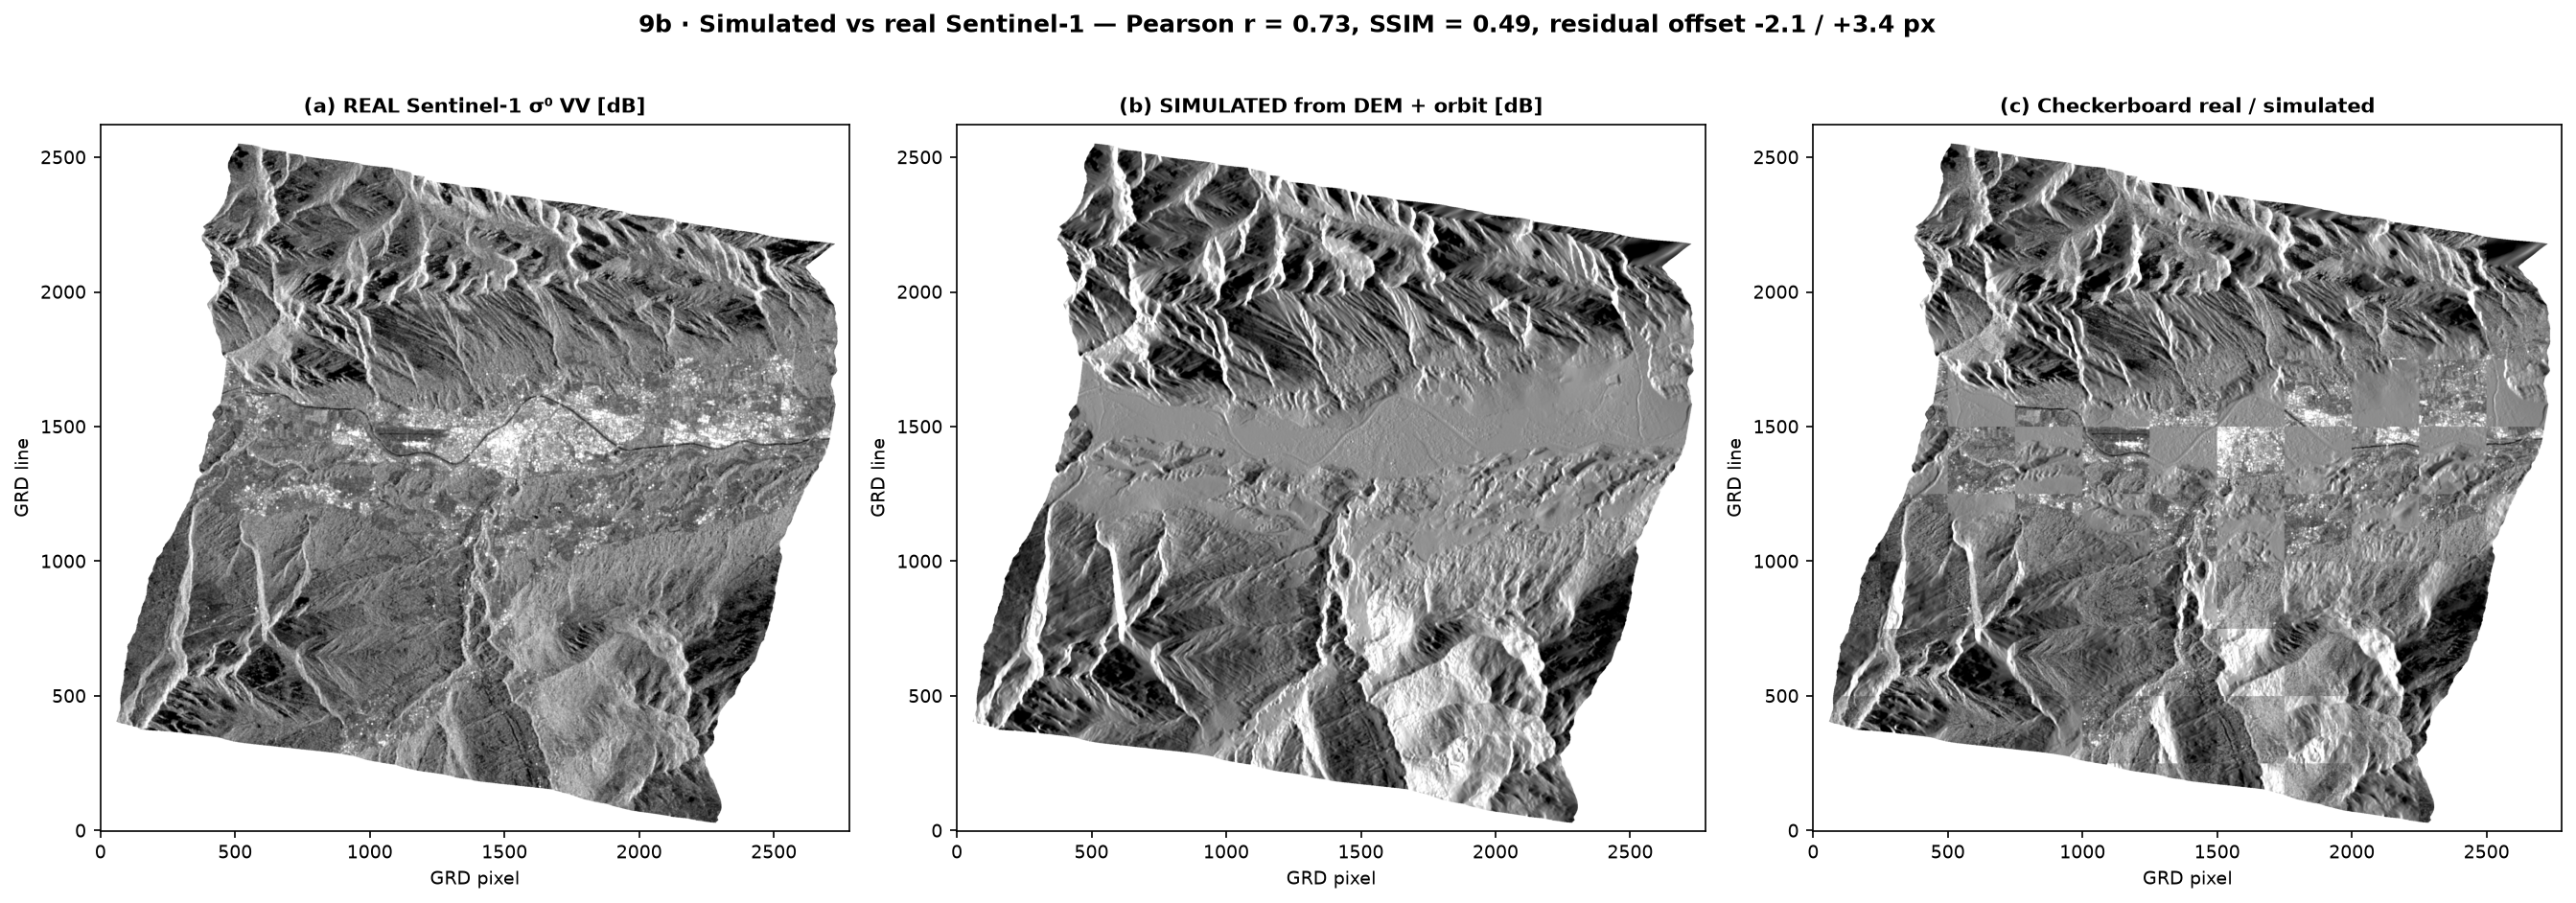
\includegraphics[width=\textwidth]{09b_real_vs_simulated.png}
\caption[Real Sentinel-1 $\sigz$, simulation with Muhleman's law and a checkerboard of both; ascending scene, radar geometry]{Real Sentinel-1 $\sigz$ (\textbf{a}), simulation with Muhleman's law (\textbf{b}) and a checkerboard of both (\textbf{c}); ascending scene, radar geometry.}
\label{fig:realsim}
\end{figure}

\begin{table}[htbp]
\caption[Agreement between the real and the simulated ascending image for five backscatter laws ($5\times5$ multilook, dB)]{Agreement between the real and the simulated ascending image for five backscatter laws ($5\times5$ multilook, dB). The level offset is the constant added to the law to calibrate its absolute level.}
\label{tab:models}
\centering\small
\begin{tabular}{lrrrrr}\toprule
 Backscatter model & Pearson $r$ & Spearman $\rho$ & SSIM & RMSE [dB] & level offset [dB]\\\midrule
Constant & 0.534 & 0.739 & 0.377 & 3.83 & -0.6 \\
$\cos\theta_{loc}$ & 0.663 & 0.767 & 0.467 & 3.72 & -8.3 \\
$\cos^2\theta_{loc}$ (Lambert) & 0.703 & 0.762 & 0.509 & 4.44 & -6.1 \\
Muhleman & 0.734 & 0.757 & 0.494 & 4.58 & 7.6 \\
Fitted $k\cos^{1.98}\theta_{loc}$ & 0.710 & 0.761 & 0.508 & 4.29 & -1.4 \\
\bottomrule\end{tabular}

\end{table}

\begin{figure}[htbp]
\centering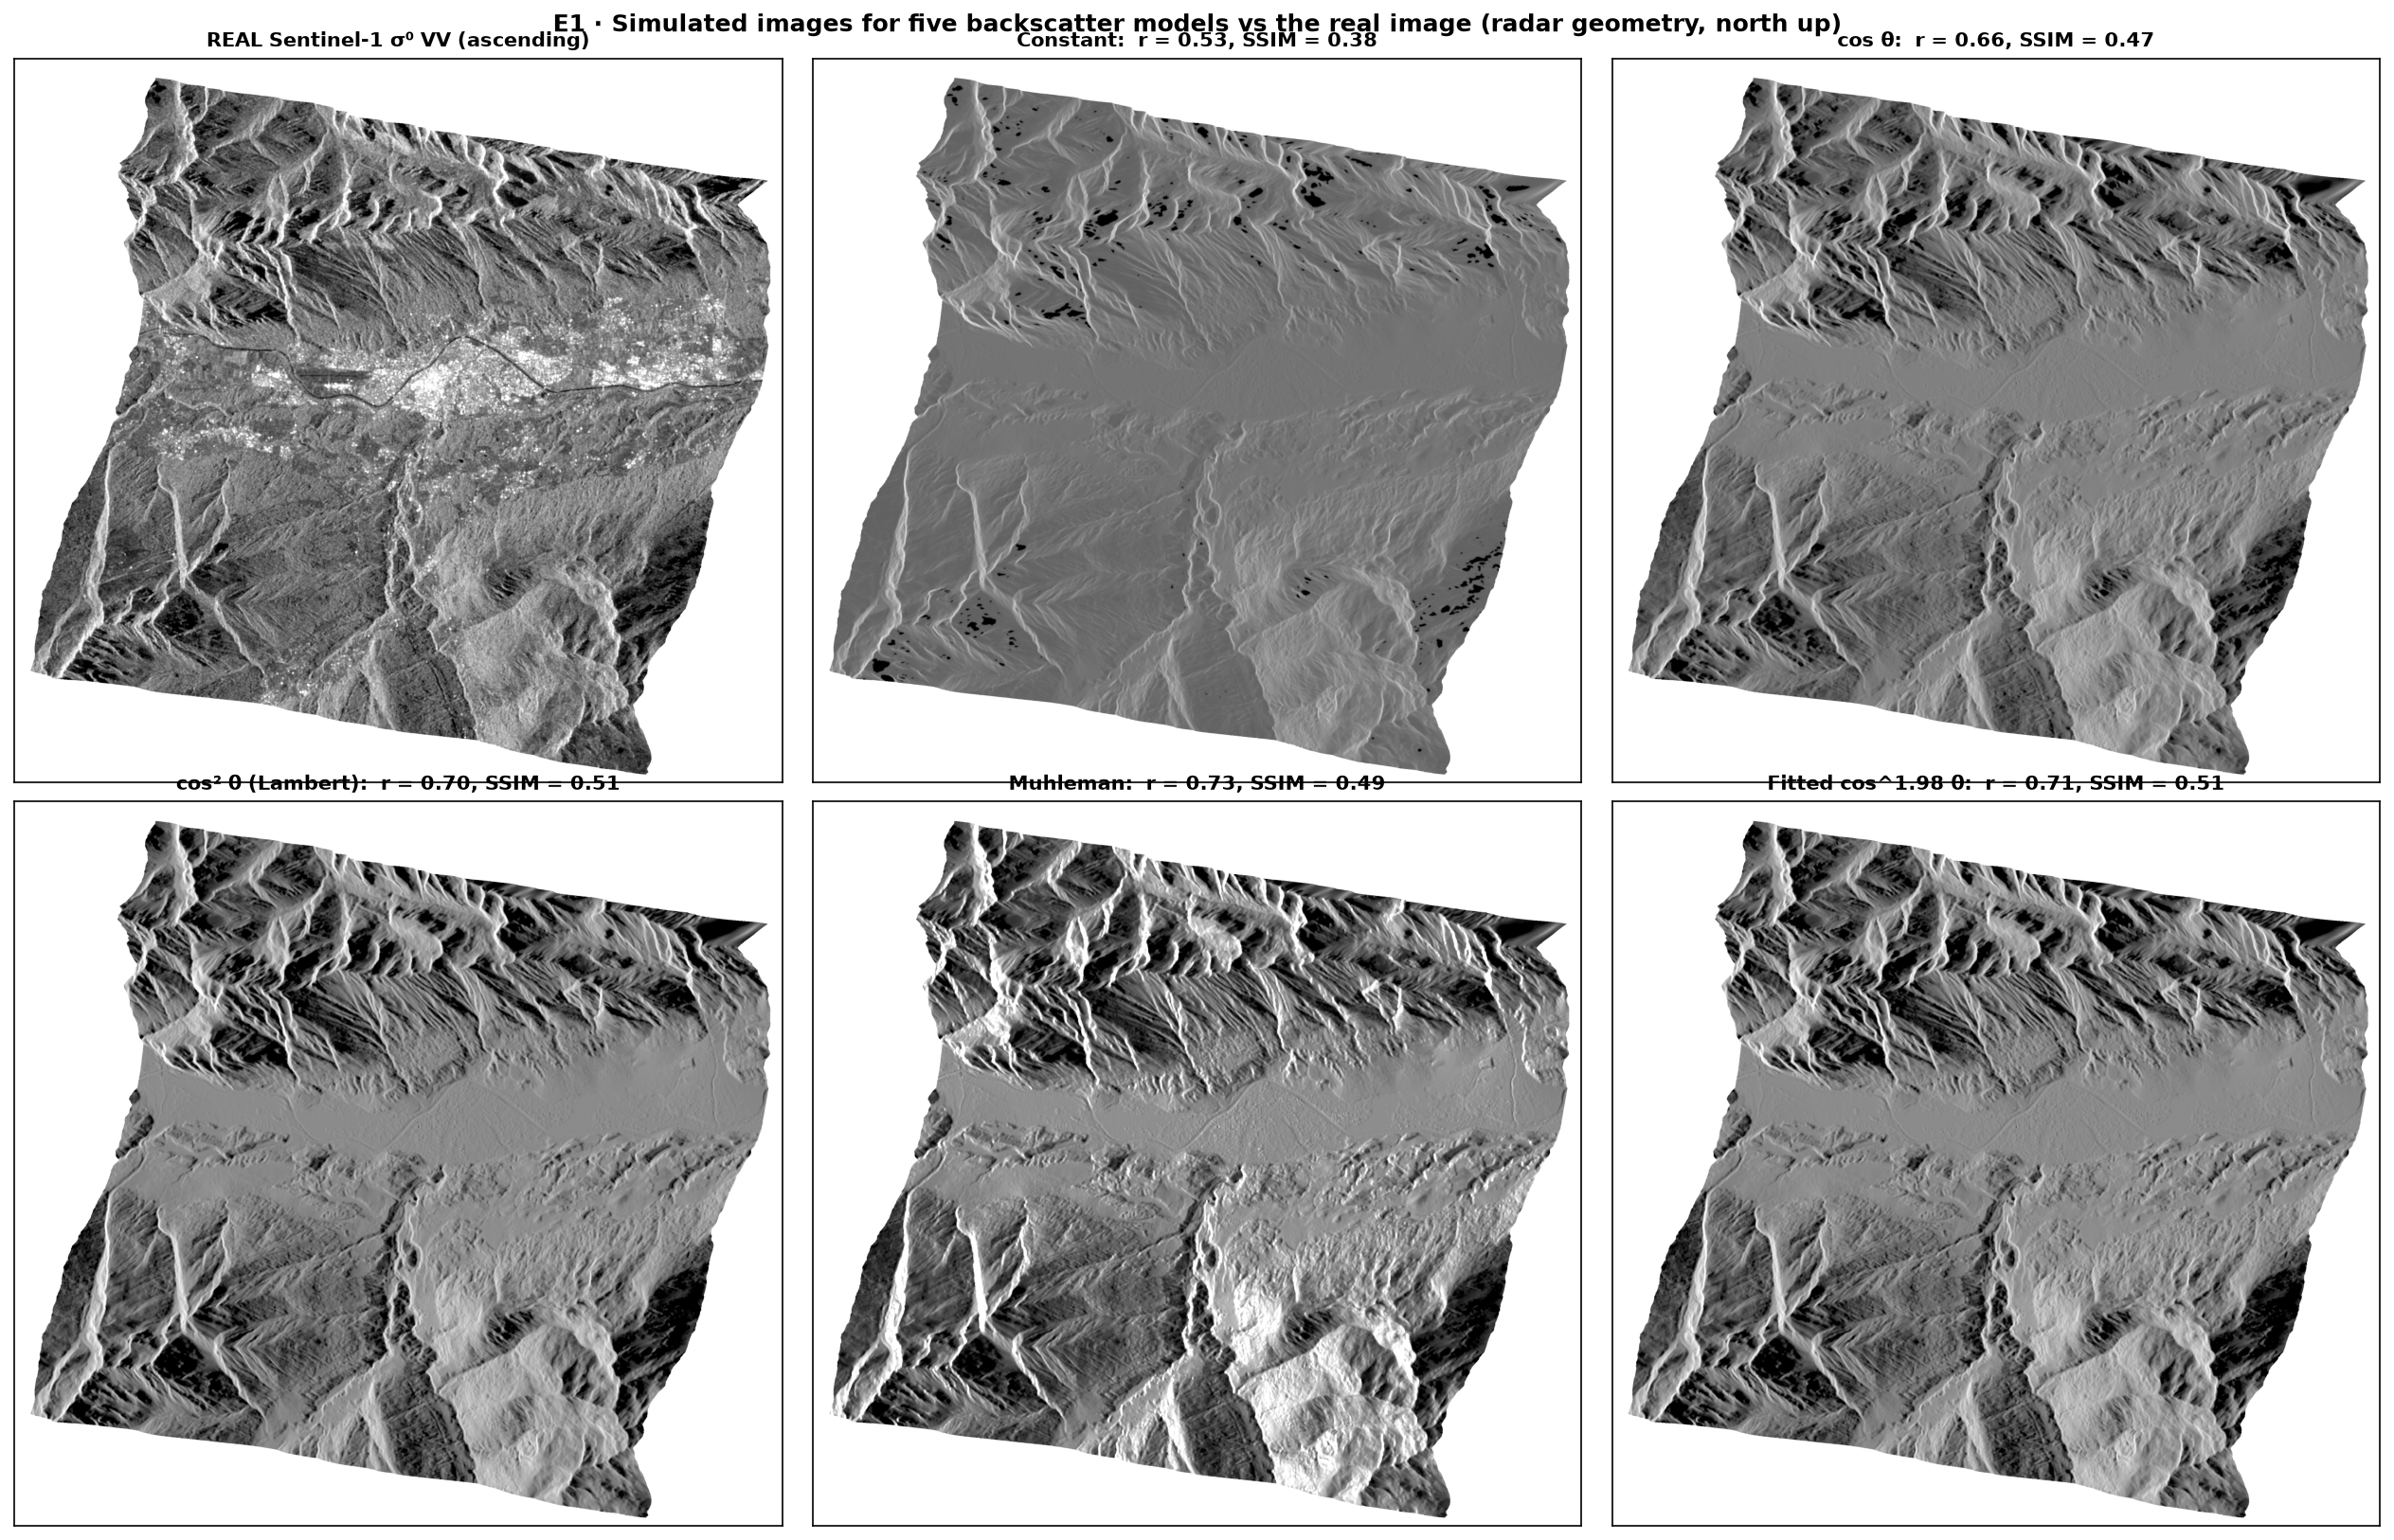
\includegraphics[width=\textwidth]{p1_models_images.png}
\caption[Real ascending image and simulations with the five backscatter laws (radar geometry, north up)]{Real ascending image and simulations with the five backscatter laws (radar geometry, north up).}
\label{fig:models}
\end{figure}
\begin{figure}[htbp]
\centering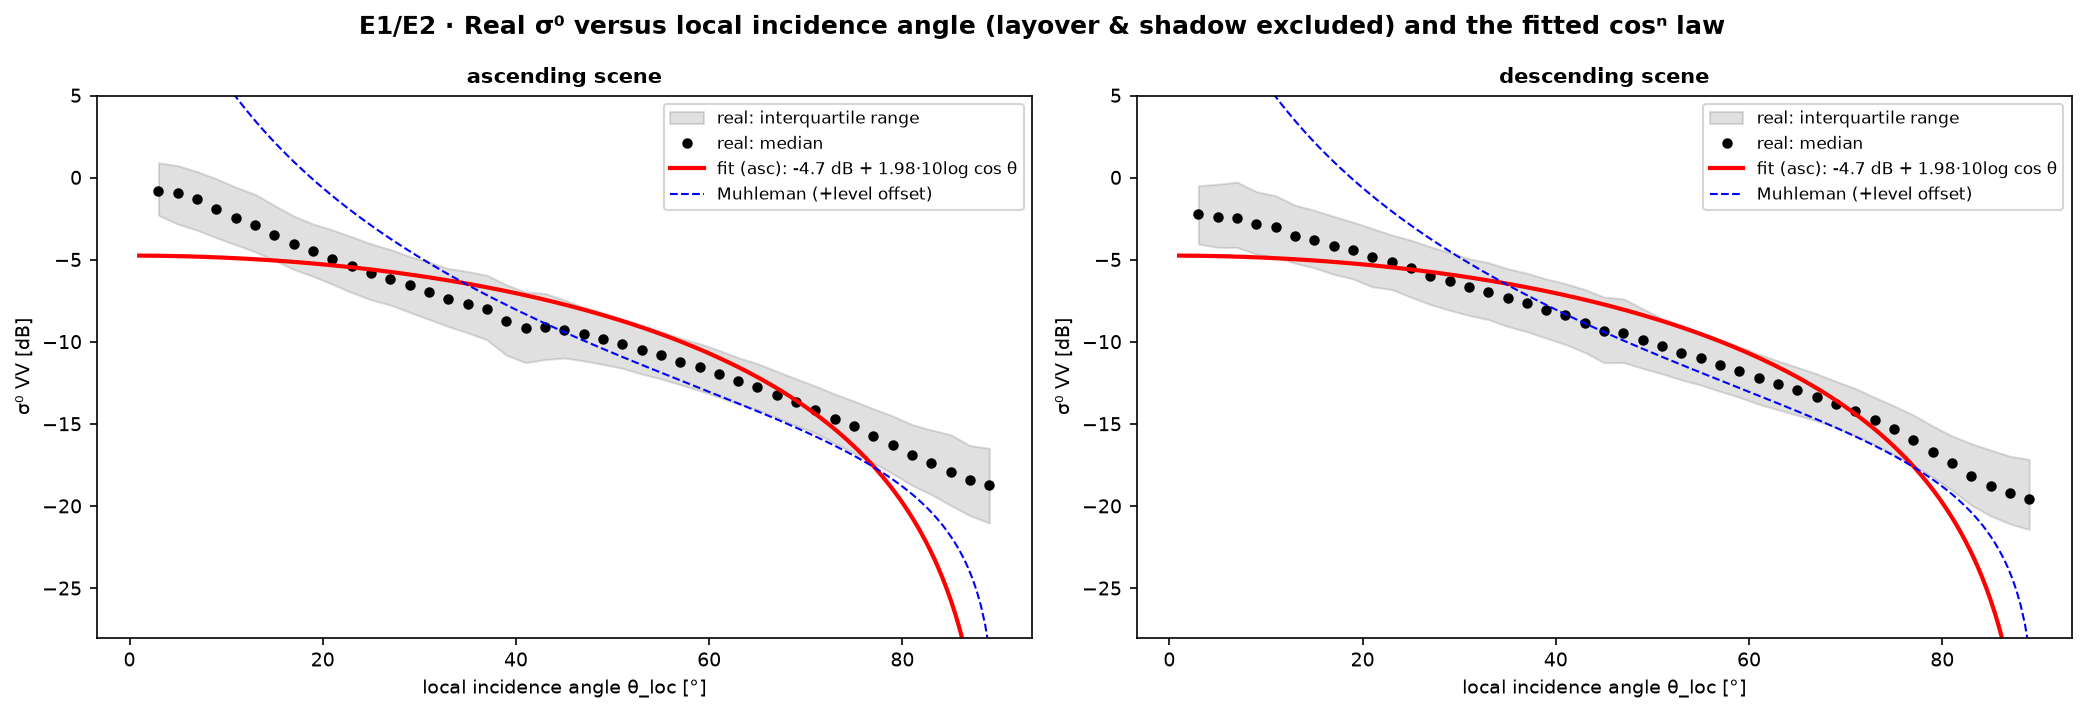
\includegraphics[width=\textwidth]{p2_fitted_model.png}
\caption[Real $\sigz$ as a function of the local incidence angle for the ascending and descending scenes, excluding layover and shadow, with the $\cos^n$ law fitted on the ascending scene and Muhleman's law]{Real $\sigz$ as a function of the local incidence angle for the ascending (\textbf{a}) and descending (\textbf{b}) scenes, excluding layover and shadow, with the $\cos^n$ law fitted on the ascending scene and Muhleman's law.}
\label{fig:fit}
\end{figure}

\section{Second Viewing Geometry}
The descending scene looks west, so that layover and shadow move to the opposite slopes (Fig.~\ref{fig:ascdesc}). Applying the law fitted on the ascending scene without any change yields $r=\rDesc$, $\rho=\rhoDesc$, SSIM\,$=\ssimDesc$ and RMSE\,$=\rmseDesc$\,dB, compared with $r=\rAsc$, $\rho=\rhoAsc$, SSIM\,$=\ssimAsc$ and RMSE\,$=\rmseAsc$\,dB on the ascending scene (Fig.~\ref{fig:scatter}). A refit on the descending scene gives $n=\nRefitDesc$. The empirical law therefore transfers between the two viewing geometries; it describes the terrain rather than the acquisition.

\begin{figure}[htbp]
\centering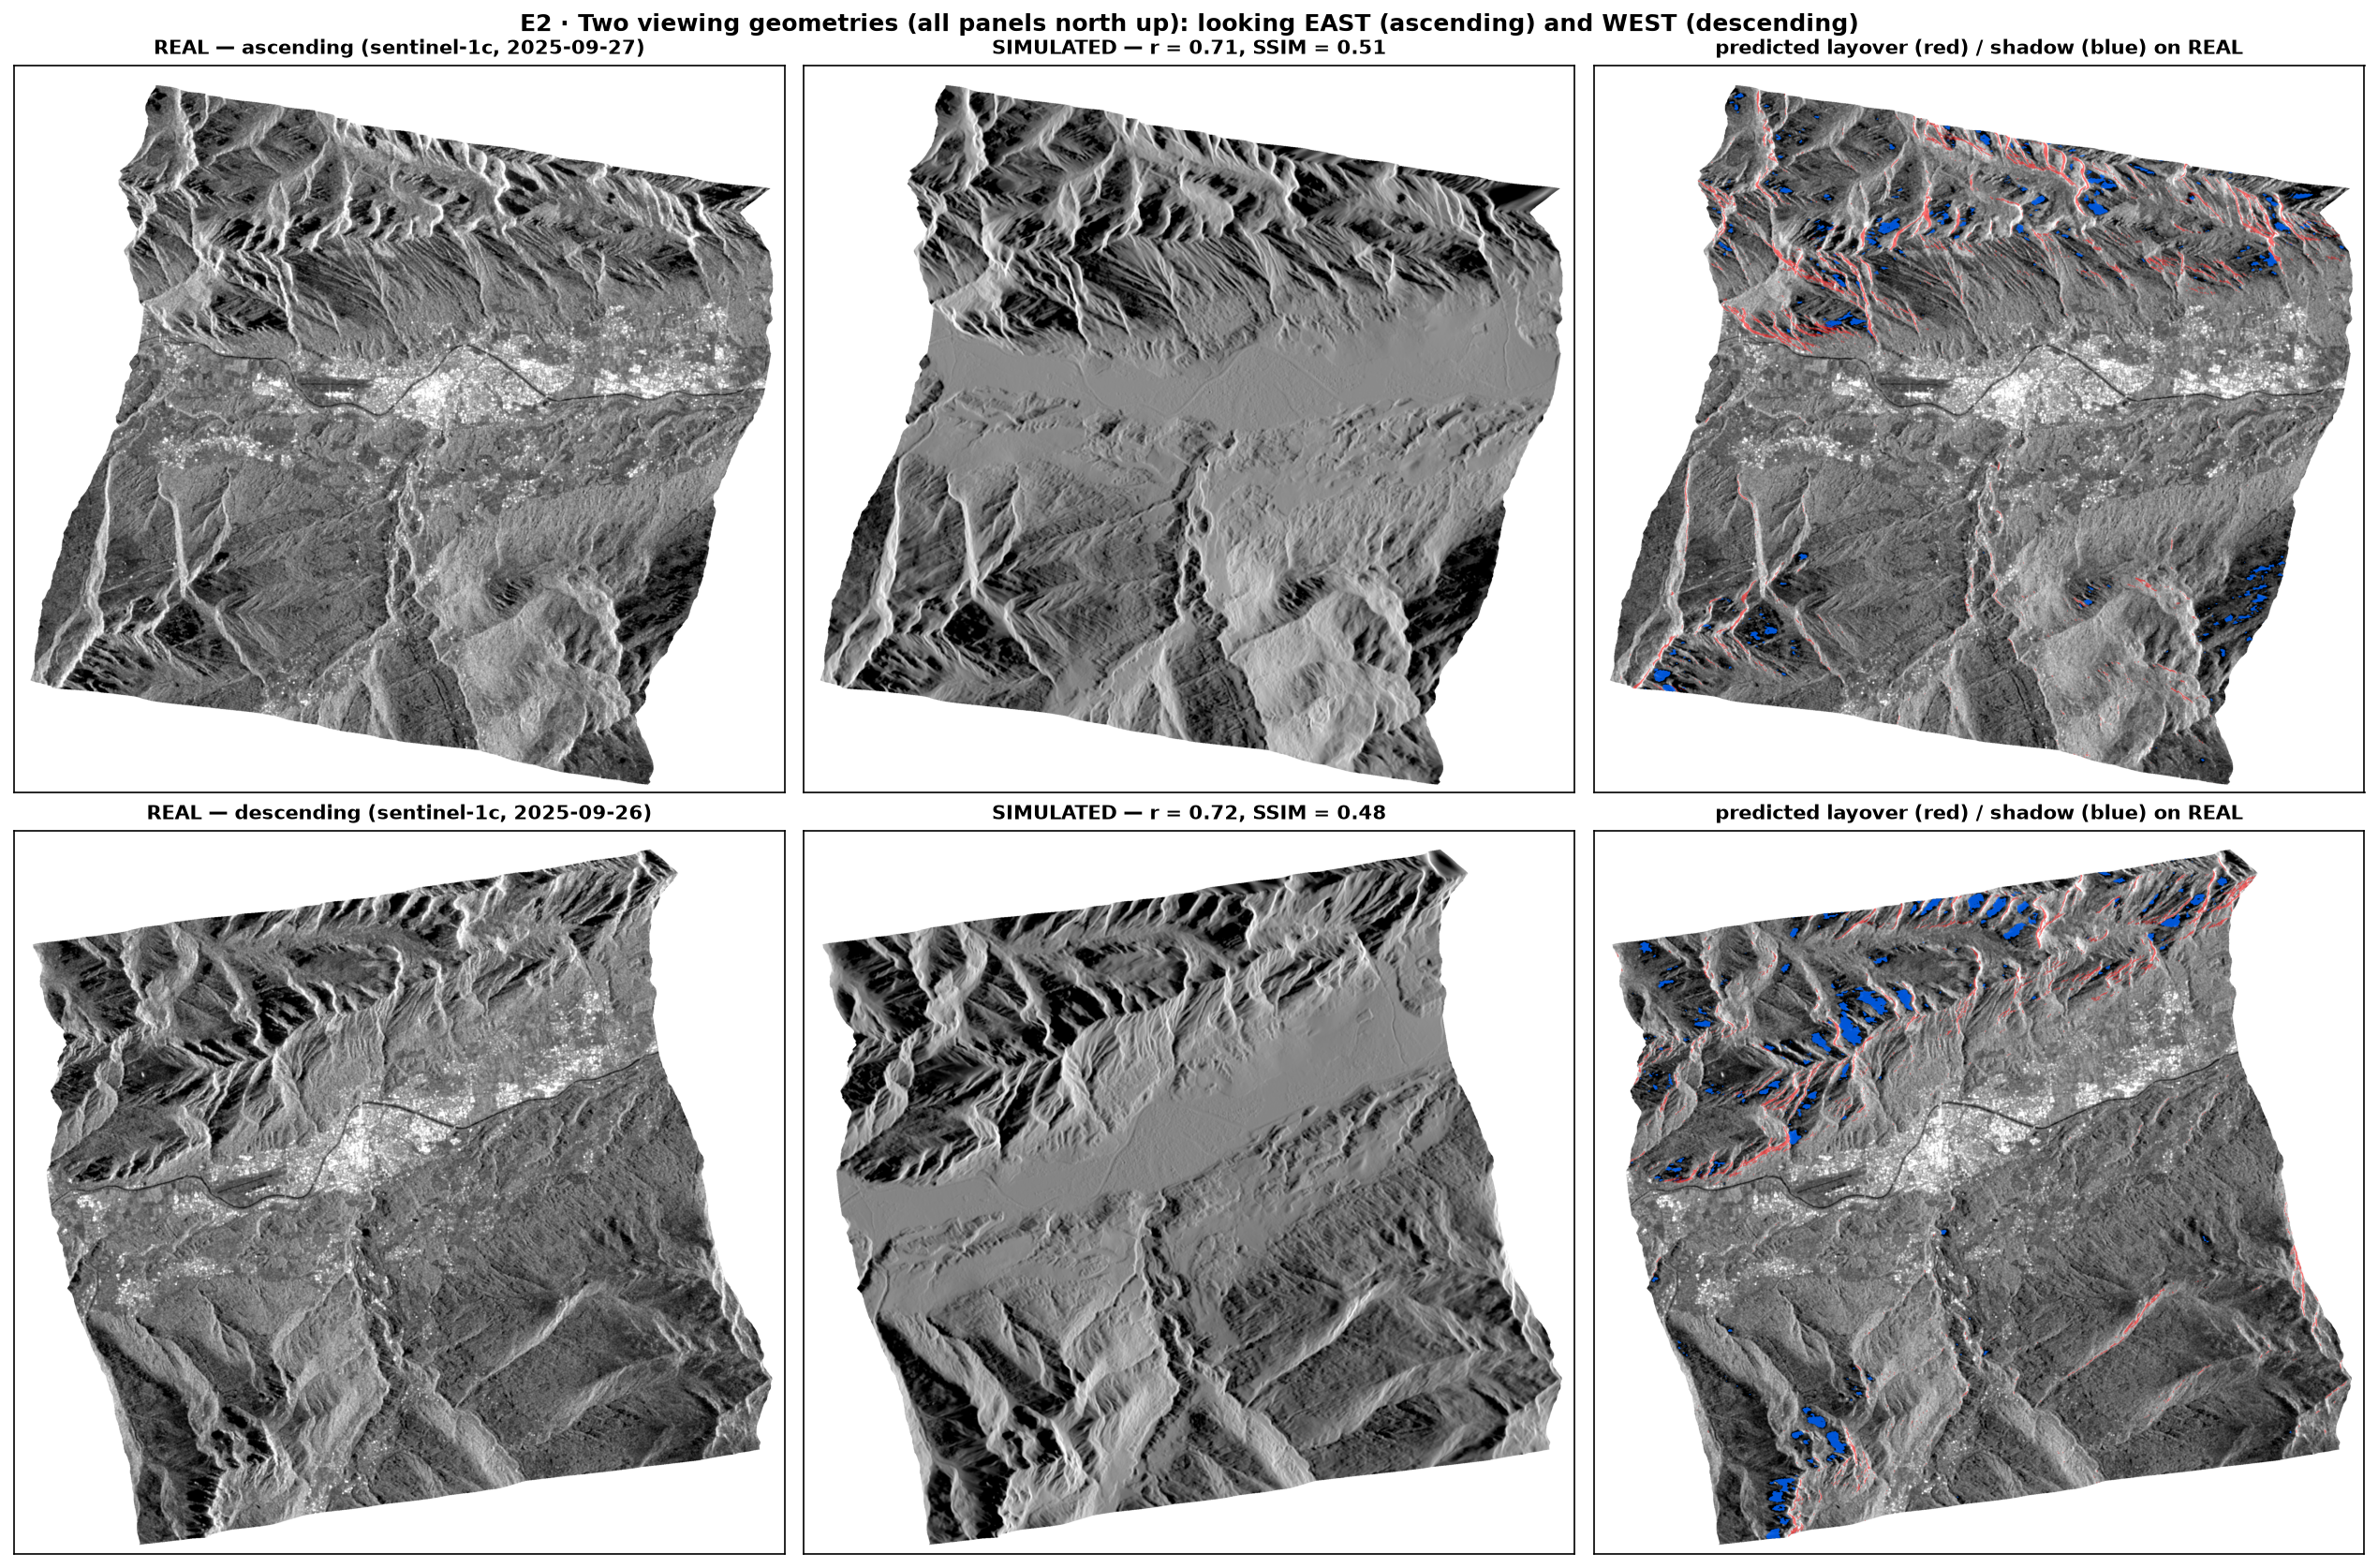
\includegraphics[width=\textwidth]{p3_ascending_descending.png}
\caption[Real and simulated images, and predicted layover (red) and shadow (blue) drawn on the real image, for the ascending (top, looking east) and descending (bottom, looking west) scenes; all panels north up]{Real and simulated images, and predicted layover (red) and shadow (blue) drawn on the real image, for the ascending (top, looking east) and descending (bottom, looking west) scenes; all panels north up.}
\label{fig:ascdesc}
\end{figure}
\begin{figure}[htbp]
\centering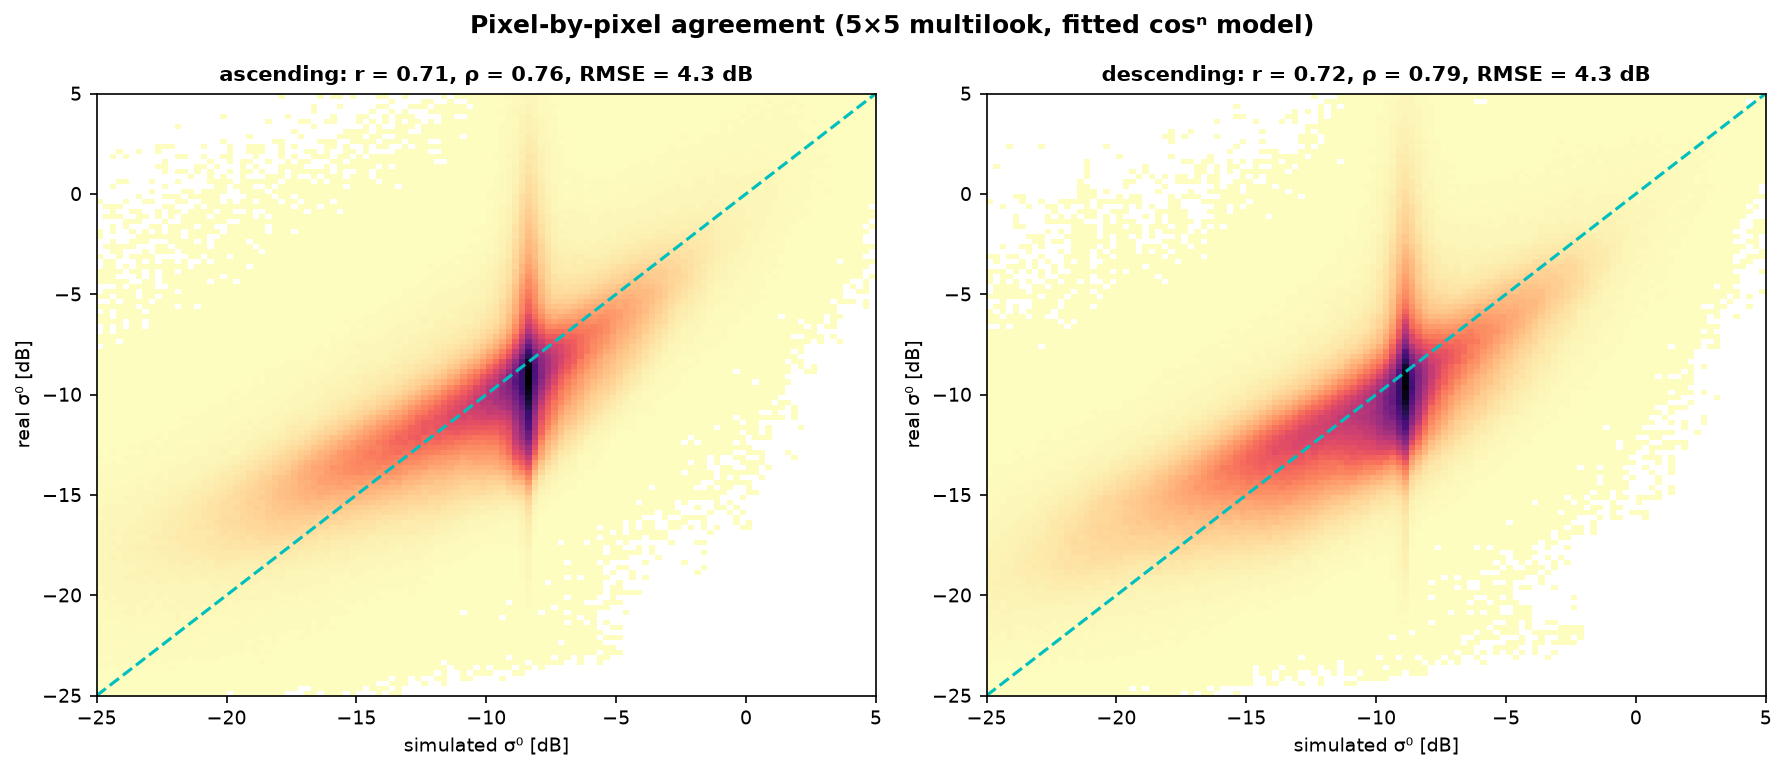
\includegraphics[width=0.86\textwidth]{p8_scatter.png}
\caption[Pixel-by-pixel comparison of real and simulated $\sigz$ for both scenes with the fitted law]{Pixel-by-pixel comparison of real and simulated $\sigz$ for both scenes with the fitted law.}
\label{fig:scatter}
\end{figure}

\section{Validation of the Predicted Distortion Classes}
Table~\ref{tab:classes} and Fig.~\ref{fig:geomval} test the predicted distortion classes against the real images. Pixels predicted to be in shadow are the darkest, with a median of $-21.0$\,dB (ascending) and $-22.0$\,dB (descending), i.e., at the noise floor of the sensor, since thermal noise was not removed. Pixels predicted to be in layover ($-3.5$ and $-3.9$\,dB) or strongly foreshortened ($-4.5$ and $-5.1$\,dB) are the brightest, about 7\,dB above the remaining terrain. The ordering of the classes is identical in both geometries.

\begin{table}[htbp]
\caption[Real $\sigz$ inside the distortion classes predicted by the simulation]{Real $\sigz$ inside the distortion classes predicted by the simulation.}
\label{tab:classes}
\centering\small
\begin{tabular}{lrrrr}\toprule
 & \multicolumn{2}{c}{ascending} & \multicolumn{2}{c}{descending}\\
Predicted class & pixels & median $\sigma^0$ [dB] & pixels & median $\sigma^0$ [dB]\\\midrule
shadow & 47k & -21.0 & 66k & -22.0 \\
layover & 82k & -3.5 & 61k & -3.9 \\
foreshortened (area > 2x) & 228k & -4.5 & 220k & -5.1 \\
other terrain & 4525k & -10.8 & 4576k & -11.5 \\
\bottomrule\end{tabular}

\end{table}
\begin{figure}[htbp]
\centering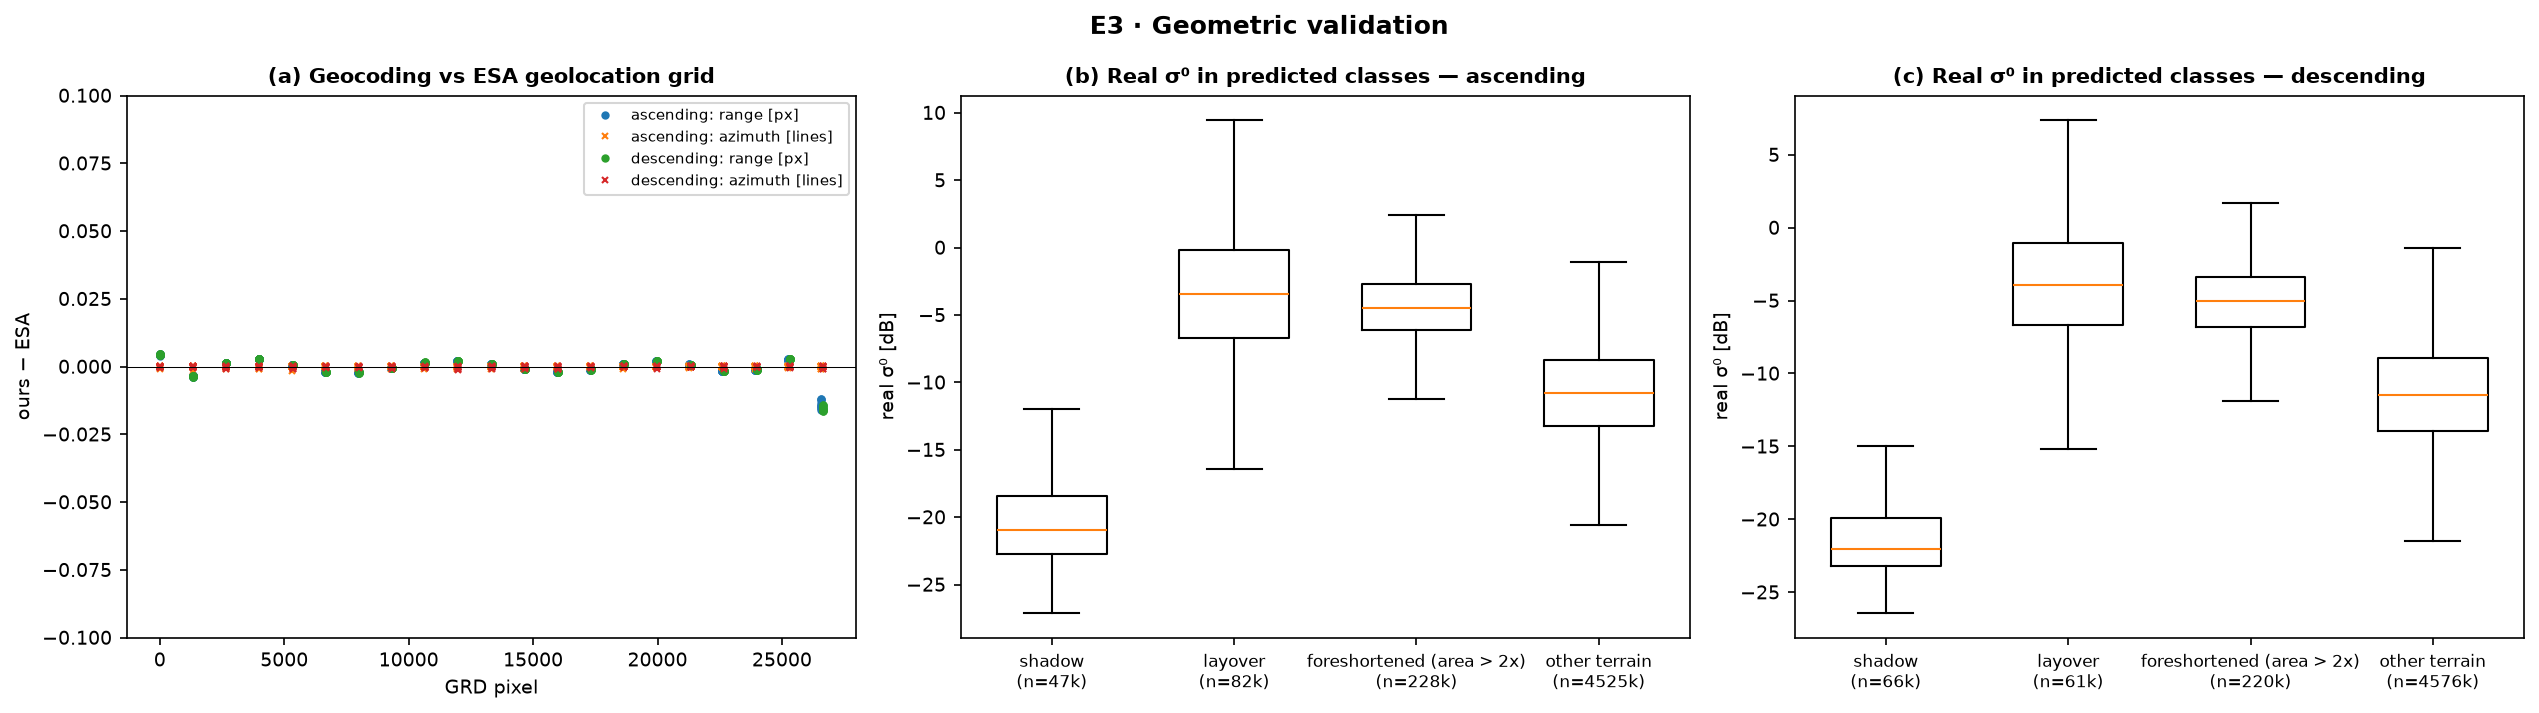
\includegraphics[width=\textwidth]{p4_geometric_validation.png}
\caption[Geometric validation]{Geometric validation: (\textbf{a}) geocoding residuals with respect to the geolocation grid of both products; (\textbf{b},\textbf{c}) real $\sigz$ in the predicted classes for the ascending and descending scenes.}
\label{fig:geomval}
\end{figure}

\section{Sensitivity to Processing Choices}
Table~\ref{tab:sens} and Fig.~\ref{fig:sens} vary one processing choice at a time. Omitting the geoid correction ($N=\geoidN$\,m) moves the simulation by 5.8 pixels (58\,m) in range, in agreement with the expected ground-range displacement $N/\tan\theta$ of about 61\,m of a height error $N$ at an incidence angle of about 39$^\circ$; co-registration absorbs this shift and the correlation is unchanged, but an un-co-registered product such as a layover and shadow mask would be misplaced by six pixels. Without DEM oversampling, \holesNoOver\,\% of the GRD pixels receive no facet, compared with \holesBase\,\% with threefold oversampling, in a striped pattern on all slopes facing away from the radar. After $5\times5$ multilooking the correlation hardly changes ($r=\rNoOver$), but single-look products and masks would be unusable. A 90\,m DEM gives the same correlation as GLO-30 ($r=\rDemNinety$): at the 50\,m scale of the comparison, the large landforms dominate, and the finer DEM matters for full-resolution products.

\begin{table}[htbp]
\caption[Sensitivity of the simulation (ascending scene, fitted law)]{Sensitivity of the simulation (ascending scene, fitted law). $\Delta$line and $\Delta$pixel are the residual shifts found by co-registration.}
\label{tab:sens}
\centering\small
\resizebox{\textwidth}{!}{\begin{tabular}{lrrrrr}\toprule
 Configuration & $r$ & SSIM & $\Delta$line & $\Delta$pixel & empty px [\%]\\\midrule
baseline (GLO-30, 3x oversampled, geoid) & 0.710 & 0.508 & -2.2 & 3.5 & 0.01 \\
no geoid correction (N = 0) & 0.710 & 0.507 & -2.2 & -2.3 & 0.01 \\
no DEM oversampling & 0.706 & 0.446 & -2.2 & 3.5 & 45.82 \\
90 m DEM (GLO-30 aggregated 3x3) & 0.714 & 0.418 & -2.3 & 3.5 & 0.00 \\
\bottomrule\end{tabular}
}
\end{table}
\begin{figure}[htbp]
\centering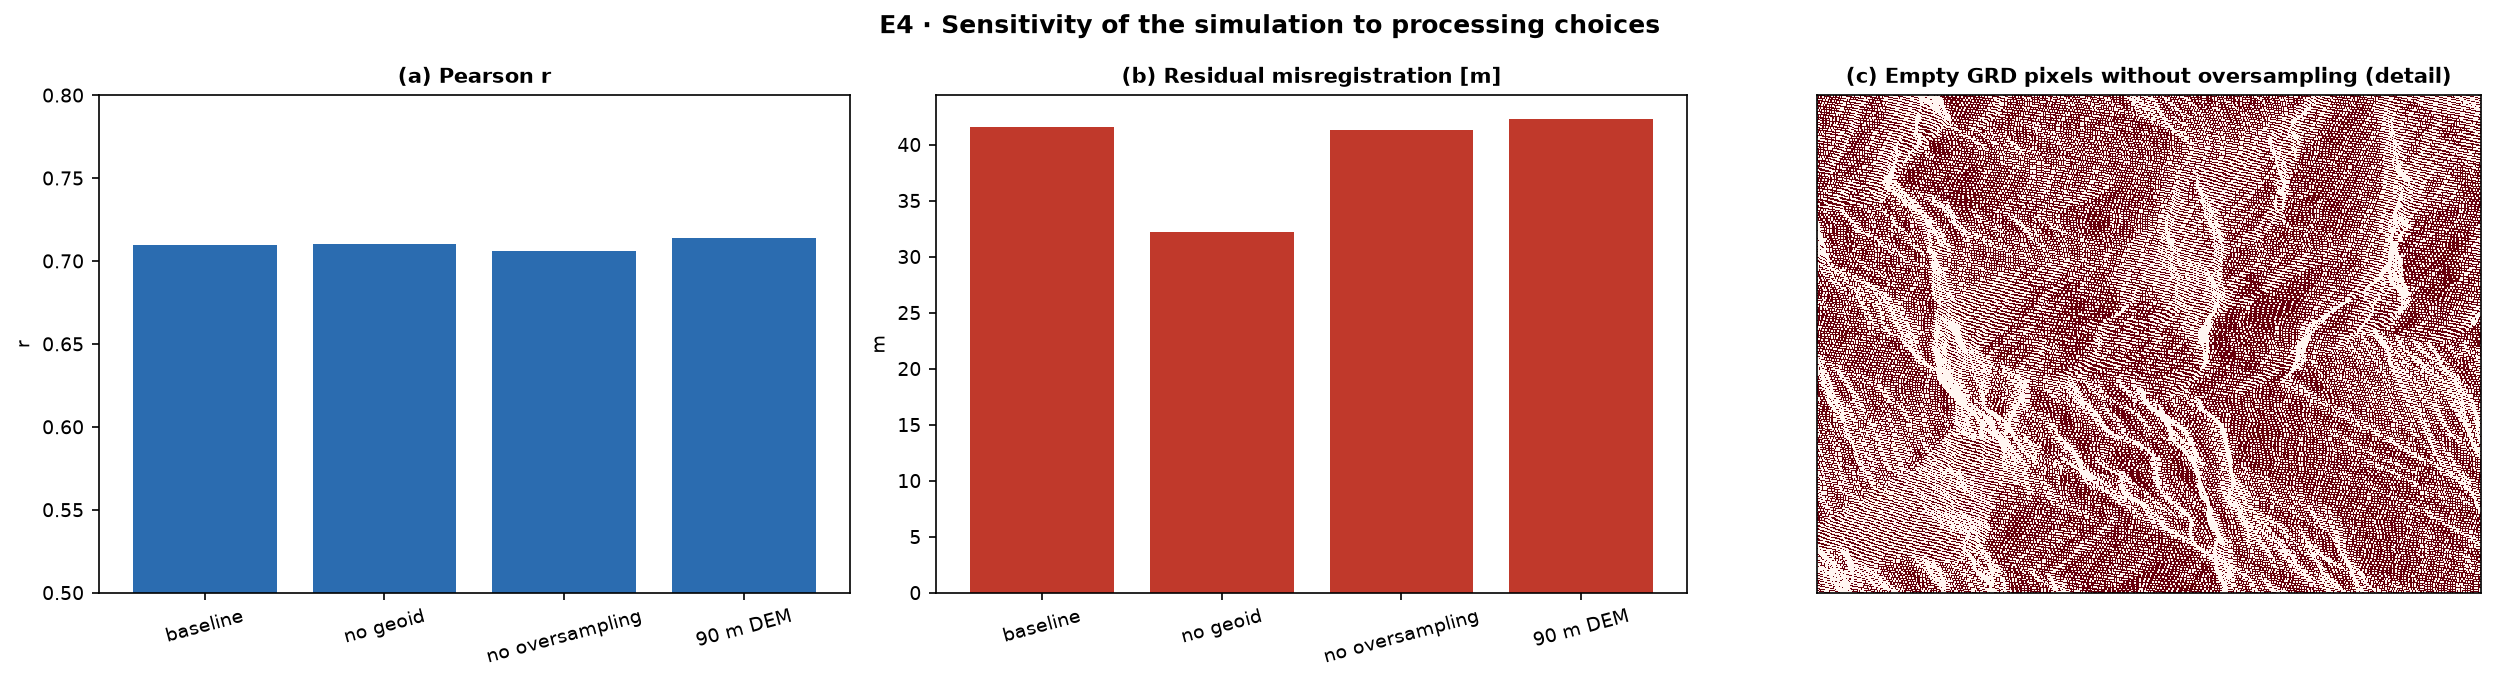
\includegraphics[width=\textwidth]{p5_sensitivity.png}
\caption[Sensitivity]{Sensitivity: (\textbf{a}) correlation; (\textbf{b}) residual misregistration; (\textbf{c}) GRD pixels that receive no facet without DEM oversampling (detail of the Nordkette).}
\label{fig:sens}
\end{figure}

\section{Contribution of Land Cover}
Grouping the residuals by WorldCover class (Table~\ref{tab:lc}, Figs.~\ref{fig:lc} and~\ref{fig:resmap}) shows where a DEM-only simulation fails. Tree cover, which represents 55\,\% of the area, is reproduced without bias ($-0.1$\,dB) and with the highest correlation ($r=0.86$): the volume scattering of the forest canopy is close to the smooth angular law fitted to a scene that forest dominates. Built-up areas ($+3.1$\,dB) are brighter than predicted because double-bounce reflections between walls and the ground are absent from any facet model~\cite{balz2009,auer2010}; bare rock and scree ($+3.2$\,dB) are rougher than the average surface. Water ($-3.8$\,dB), cropland ($-2.0$\,dB) and grassland ($-1.4$\,dB) are darker because smooth surfaces reflect specularly away from the radar~\cite{ulaby1982}. The low correlations within the built-up, cropland and water classes ($r=0.22$--$0.30$) do not indicate a geometric failure: these classes lie on the flat valley floor, where the DEM predicts an almost constant value and the terrain signal to correlate with is weak.

\begin{table}[htbp]
\caption[Residual (real minus simulated $\sigz$) and correlation per land-cover class (ascending scene, map geometry, layover and shadow excluded)]{Residual (real minus simulated $\sigz$) and correlation per land-cover class (ascending scene, map geometry, layover and shadow excluded).}
\label{tab:lc}
\centering\small
\begin{tabular}{lrrrr}\toprule
 WorldCover class & area [\%] & mean residual [dB] & std [dB] & $r$\\\midrule
Tree cover & 55.3 & -0.14 & 2.52 & 0.86 \\
Grassland & 25.9 & -1.44 & 3.28 & 0.77 \\
Cropland & 3.9 & -2.00 & 2.54 & 0.23 \\
Built-up & 7.2 & 3.11 & 4.54 & 0.22 \\
Bare / sparse & 5.8 & 3.18 & 4.29 & 0.82 \\
Snow \& ice & 0.3 & 2.09 & 2.91 & 0.86 \\
Water & 0.5 & -3.76 & 4.12 & 0.30 \\
Moss \& lichen & 1.2 & 0.51 & 3.27 & 0.88 \\
\bottomrule\end{tabular}

\end{table}
\begin{figure}[htbp]
\centering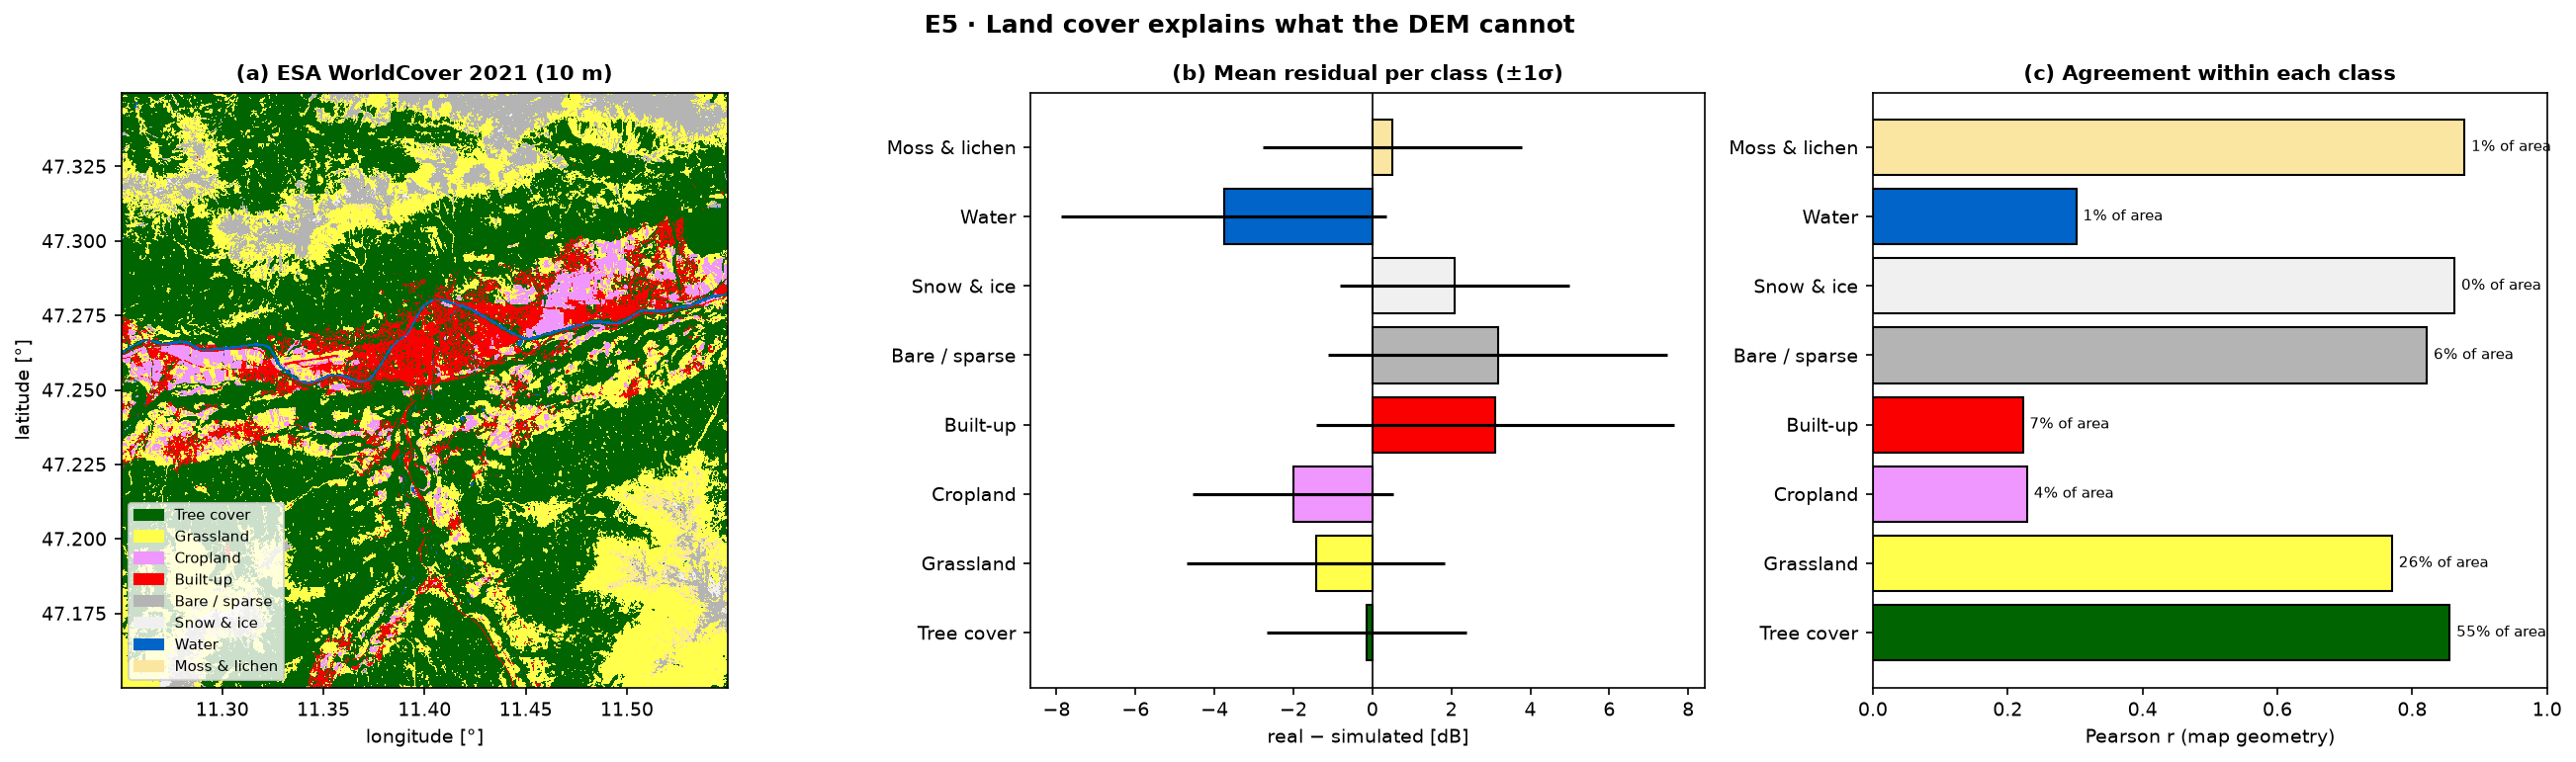
\includegraphics[width=\textwidth]{p6_landcover.png}
\caption[Land cover]{Land cover: (\textbf{a}) ESA WorldCover map of the study site; (\textbf{b}) mean residual per class ($\pm1$ standard deviation); (\textbf{c}) correlation within each class.}
\label{fig:lc}
\end{figure}
\begin{figure}[htbp]
\centering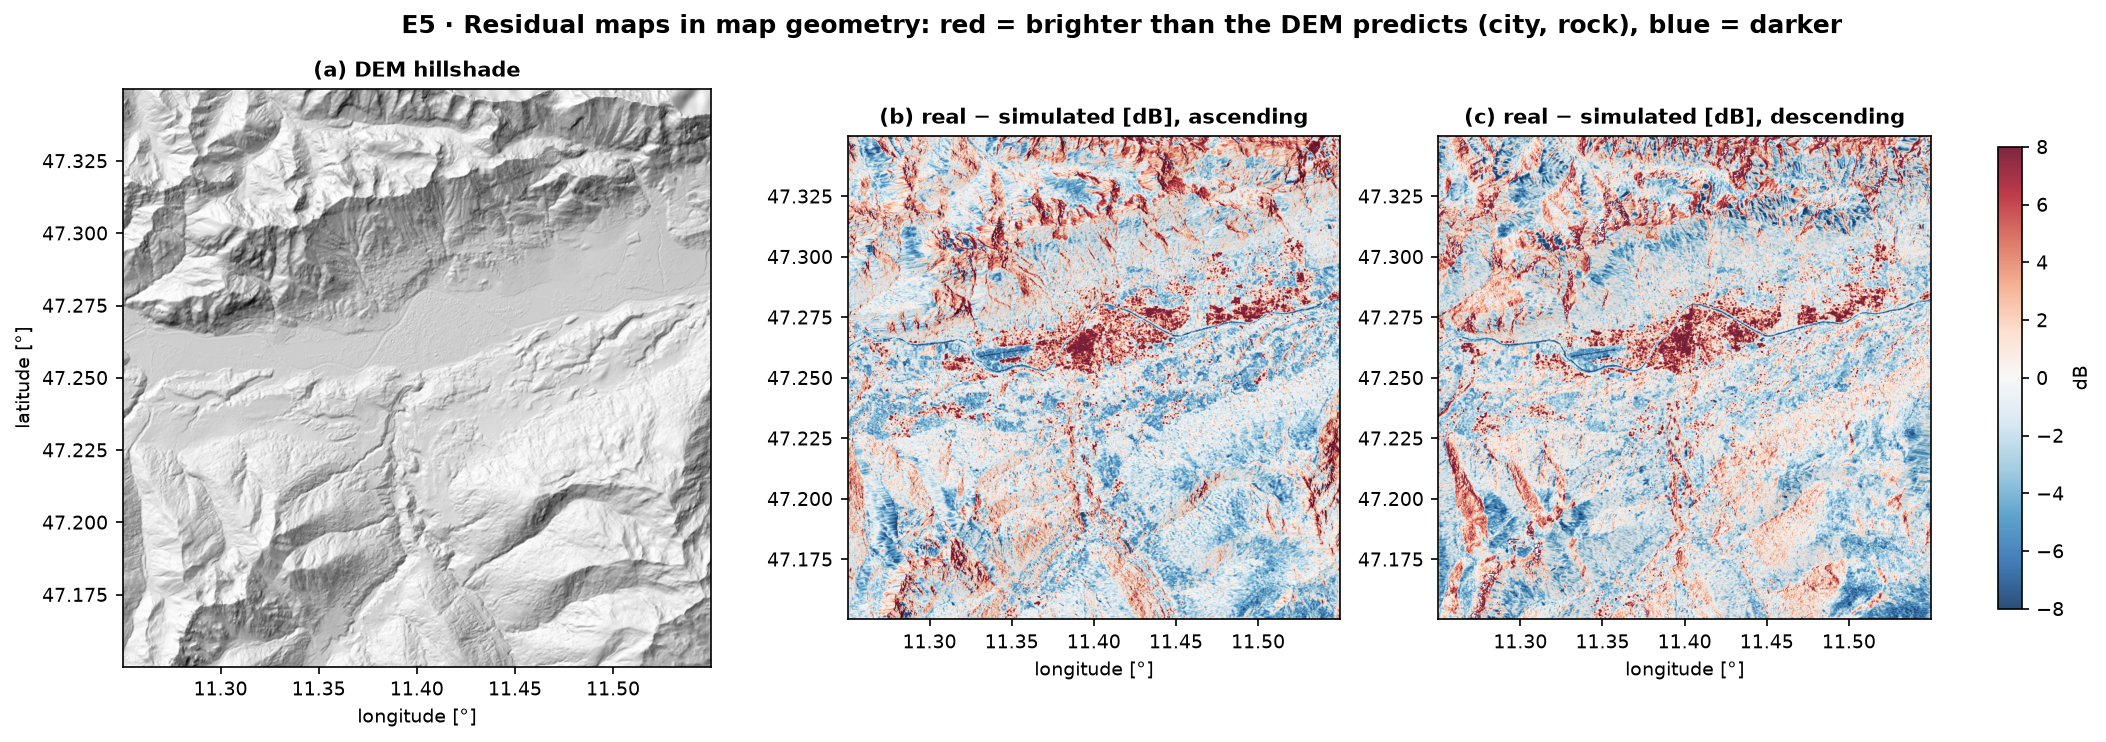
\includegraphics[width=\textwidth]{p7_residual_maps.png}
\caption[DEM hillshade and residual maps (real minus simulated $\sigz$) in map geometry for the ascending and descending scenes]{DEM hillshade (\textbf{a}) and residual maps (real minus simulated $\sigz$) in map geometry for the ascending (\textbf{b}) and descending (\textbf{c}) scenes.}
\label{fig:resmap}
\end{figure}

\section{Limitations of the Study}
The results presented in this section show that terrain geometry explains a large part of Sentinel-1 images of Alpine terrain. A few limitations related to the data and the methodology should nevertheless be discussed.

First, co-registration still finds offsets between image and simulation of \shiftAscL{} lines and \shiftAscP{} pixels (about 22\,m in azimuth and 35\,m in range) for the ascending scene and \shiftDescL{} lines and \shiftDescP{} pixels for the descending scene. Because the geocoding reproduces the product annotation to a small fraction of a pixel, these offsets measure the discrepancy between the image content and the annotated geolocation of the products, combined with DEM errors on steep slopes. Atmospheric path delay, solid-earth tides and the orbit used for near-real-time products, which are not modelled here, are known to contribute to the absolute geolocation error of Sentinel-1~\cite{schubert2015,gisinger2021}. Such offsets are routinely removed by simulation-based co-registration~\cite{nitti2011,small2011}.

Second, the simulator is an incoherent single-bounce model. It does not represent double bounce, volume scattering or multipath, which explains the residuals over built-up areas and the spread of real $\sigz$ at a given local incidence angle. Third, thermal noise was not removed, so that predicted shadow is compared with the noise floor rather than with zero. Fourth, one date per geometry was used; seasonal effects such as snow cover or soil moisture, and the time difference between the DEM acquisitions and the 2025 images, were not analysed. Finally, the absolute level of each backscatter law was calibrated by a constant; absolute radiometric prediction would require a land-cover-dependent model. These limitations do not affect the geometric conclusions of this study.
